%%%%%%%% ICML 2026 EXAMPLE LATEX SUBMISSION FILE %%%%%%%%%%%%%%%%%

\documentclass{article}

% XeLaTeX typography for the Chinese translation.
\usepackage[UTF8,fontset=none,heading=false]{ctex}
\setCJKmainfont[AutoFakeBold=2.5,ItalicFont={Songti SC}]{Songti SC}
\setCJKsansfont[AutoFakeBold=2.5]{Hiragino Sans GB}
\setCJKmonofont[Scale=0.92]{Hiragino Sans GB}
\XeTeXlinebreaklocale "zh"
\XeTeXlinebreakskip = 0pt plus 1pt

% Recommended, but optional, packages for figures and better typesetting:
\usepackage{microtype}
\usepackage{graphicx}
\usepackage{subcaption}
\usepackage{booktabs} % for professional tables

% hyperref makes hyperlinks in the resulting PDF.
% If your build breaks (sometimes temporarily if a hyperlink spans a page)
% please comment out the following usepackage line and replace
% \usepackage{icml2026} with \usepackage[nohyperref]{icml2026} above.
\usepackage{hyperref}
\usepackage{multirow}


\usepackage[table]{xcolor}
\definecolor{MBlue}{HTML}{A4C2E6} 
\definecolor{MPink}{HTML}{E8C2C0}
\definecolor{MGray}{HTML}{F4F5F7}  
\newcommand{\bg}[2][0]{\cellcolor{MBlue!#1}#2}      
\newcommand{\bged}[2][0]{\cellcolor{MPink!#1}#2}    
\newcommand{\bgbase}[1]{\cellcolor{MGray!100}#1}    


\newcommand{\sd}[2]{{#1}_{\pm#2}}
\newcommand{\sdb}[2]{\mathbf{#1}_{\pm#2}}
\newcommand{\capbox}[2]{\protect\colorbox{#1}{\textcolor{black}{\small#2}}}
\newcommand{\caplegend}[1]{\protect\raisebox{-0.1ex}{\protect\color{#1}\rule{0.6em}{0.7em}}}


% Attempt to make hyperref and algorithmic work together better:
\newcommand{\theHalgorithm}{\arabic{algorithm}}

% Use the following line for the initial blind version submitted for review:
\usepackage[accepted]{icml2026_zh}

\setmainfont{texgyretermes-regular.otf}[
  BoldFont=texgyretermes-bold.otf,
  ItalicFont=texgyretermes-italic.otf,
  BoldItalicFont=texgyretermes-bolditalic.otf
]
\setsansfont{texgyreheros-regular.otf}[
  BoldFont=texgyreheros-bold.otf,
  ItalicFont=texgyreheros-italic.otf,
  BoldItalicFont=texgyreheros-bolditalic.otf
]
\setmonofont{texgyrecursor-regular.otf}[
  BoldFont=texgyrecursor-bold.otf,
  ItalicFont=texgyrecursor-italic.otf,
  BoldItalicFont=texgyrecursor-bolditalic.otf,
  Scale=MatchLowercase
]
\renewcommand{\figurename}{图}
\renewcommand{\tablename}{表}
\captionsetup[figure]{name=图}
\captionsetup[table]{name=表}
\renewcommand{\refname}{参考文献}
\renewcommand{\appendixname}{附录}

% For preprint, use
% \usepackage[preprint]{icml2026}

% If accepted, instead use the following line for the camera-ready submission:
% \usepackage[accepted]{icml2026}

\usepackage{amsmath}
\usepackage{amssymb}
\usepackage{mathtools}
\usepackage{amsthm}


\usepackage[breakable,skins]{tcolorbox}

\tcbset{
  chatbase/.style={
    enhanced,
    breakable,
    boxrule=0pt,
    frame hidden,
    sharp corners,
    left=6pt,
    right=6pt,
    top=4pt,
    bottom=4pt,
    before skip=6pt,
    after skip=6pt,
    colback=gray!4,
    borderline west={1.2pt}{0pt}{gray!60},
  }
}

% \newtcolorbox{userchat}[1][]{%
%   chatbase,
%   colback=blue!3,
%   borderline west={1.2pt}{0pt}{blue!60},
%   #1
% }

\newtcolorbox{assistantchat}[1][]{%
  chatbase,
  colback=green!3,
  borderline west={1.2pt}{0pt}{green!50!black},
  #1
}


\newtcolorbox{userchat}[1][]{%
  enhanced,
  breakable,
  boxrule=0pt,
  frame hidden,
  sharp corners,
  left=6pt,
  right=6pt,
  top=4pt,
  bottom=4pt,
  before skip=6pt,
  after skip=6pt,
  colback=gray!4,
  borderline west={1.2pt}{0pt}{gray!60},
  #1
}



% if you use cleveref..
\usepackage[capitalize,noabbrev]{cleveref}

%%%%%%%%%%%%%%%%%%%%%%%%%%%%%%%%
% THEOREMS
%%%%%%%%%%%%%%%%%%%%%%%%%%%%%%%%
\theoremstyle{plain}
\newtheorem{theorem}{定理}[section]
\newtheorem{proposition}[theorem]{命题}
\newtheorem{lemma}[theorem]{引理}
\newtheorem{corollary}[theorem]{推论}
\theoremstyle{definition}
\newtheorem{definition}[theorem]{定义}
\newtheorem{assumption}[theorem]{假设}
\theoremstyle{remark}
\newtheorem{remark}[theorem]{注}
\renewcommand{\proofname}{证明}
\crefname{theorem}{定理}{定理}
\crefname{proposition}{命题}{命题}
\crefname{lemma}{引理}{引理}
\crefname{assumption}{假设}{假设}
\floatname{algorithm}{算法}
\renewcommand{\algorithmicrequire}{\textbf{输入：}}
\renewcommand{\algorithmicensure}{\textbf{输出：}}
\renewcommand{\algorithmicend}{\textbf{结束}}
\renewcommand{\algorithmicif}{\textbf{若}}
\renewcommand{\algorithmicthen}{\textbf{则}}
\renewcommand{\algorithmicelse}{\textbf{否则}}
\renewcommand{\algorithmicfor}{\textbf{对}}
\renewcommand{\algorithmicforall}{\textbf{对所有}}
\renewcommand{\algorithmicdo}{\textbf{执行}}
\renewcommand{\algorithmicwhile}{\textbf{当}}
\renewcommand{\algorithmicloop}{\textbf{循环}}
\renewcommand{\algorithmicrepeat}{\textbf{重复}}
\renewcommand{\algorithmicuntil}{\textbf{直到}}
\renewcommand{\algorithmicinput}{\textbf{输入}}
\renewcommand{\algorithmicoutput}{\textbf{输出}}
\renewcommand{\algorithmicset}{\textbf{设置}}
\renewcommand{\algorithmictrue}{\textbf{真}}
\renewcommand{\algorithmicfalse}{\textbf{假}}
\renewcommand{\algorithmicand}{\textbf{且\ }}
\renewcommand{\algorithmicor}{\textbf{或\ }}
\renewcommand{\algorithmicfunction}{\textbf{函数}}
\renewcommand{\algorithmicmain}{\textbf{主程序}}
\renewcommand{\algorithmicendfor}{\textbf{结束循环}}
\renewcommand{\algorithmicendwhile}{\textbf{结束循环}}
\renewcommand{\algorithmicendloop}{\textbf{结束循环}}
\renewcommand{\algorithmicendfunction}{\textbf{结束函数}}
\renewcommand{\algorithmicendmain}{\textbf{结束主程序}}

% Todonotes is useful during development; simply uncomment the next line
%    and comment out the line below the next line to turn off comments
%\usepackage[disable,textsize=tiny]{todonotes}
\usepackage[textsize=tiny]{todonotes}

% The \icmltitle you define below is probably too long as a header.
% Therefore, a short form for the running title is supplied here:
\icmltitlerunning{认知增益与偶然成本}

\begin{document}

\twocolumn[
  \icmltitle{认知增益，偶然成本：数学推理多智能体辩论中的不确定性分解}

  % It is OKAY to include author information, even for blind submissions: the
  % style file will automatically remove it for you unless you've provided
  % the [accepted] option to the icml2026 package.

  % List of affiliations: The first argument should be a (short) identifier you
  % will use later to specify author affiliations Academic affiliations
  % should list Department, University, City, Region, Country Industry
  % affiliations should list Company, City, Region, Country

  % You can specify symbols, otherwise they are numbered in order. Ideally, you
  % should not use this facility. Affiliations will be numbered in order of
  % appearance and this is the preferred way.
  \icmlsetsymbol{equal}{*}
\icmlsetsymbol{intern}{\textdagger}
\icmlsetsymbol{corr}{\textdaggerdbl}
\icmlsetsymbol{lead}{\textsection}


  \begin{icmlauthorlist}
    \icmlauthor{Dan Qiao}{sch1,sch2,intern}
    \icmlauthor{Binbin Chen}{sch2,lead}
    \icmlauthor{Fengyu Cai}{sch3}
    \icmlauthor{Jianlong Chen}{sch1}
    \icmlauthor{Wenhao Li}{sch4}
    \icmlauthor{Fuxin Jiang}{sch2}
    \icmlauthor{Zuzhi Chen}{sch2}
    \icmlauthor{Hongyuan Zha}{sch1}
    \icmlauthor{Tieying Zhang}{sch2,corr}
    \icmlauthor{Baoxiang Wang}{sch1,vector,corr}
  \end{icmlauthorlist}

% affiliation
\icmlaffiliation{sch1}{香港中文大学（深圳）数据科学学院，中国深圳}
\icmlaffiliation{sch2}{字节跳动，中国北京}
\icmlaffiliation{sch3}{达姆施塔特工业大学，德国达姆施塔特}
\icmlaffiliation{sch4}{同济大学计算机科学与技术学院，中国上海}
\icmlaffiliation{vector}{Vector 研究所}

% corresponding author
\icmlcorrespondingauthor{Baoxiang Wang}{bxwang@cuhk.edu.cn}
\icmlcorrespondingauthor{Tieying Zhang}{zhangtieying@bytedance.com} 


  % You may provide any keywords that you find helpful for describing your
  % paper; these are used to populate the "keywords" metadata in the PDF but
  % will not be shown in the document
  \icmlkeywords{多智能体辩论，不确定性分解，多智能体强化学习，数学推理}

  \vskip 0.3in
]

% this must go after the closing bracket ] following \twocolumn[ ...

% This command actually creates the footnote in the first column listing the
% affiliations and the copyright notice. The command takes one argument, which
% is text to display at the start of the footnote. The \icmlEqualContribution
% command is standard text for equal contribution. Remove it (just {}) if you
% do not need this facility.

% Use ONE of the following lines. DO NOT remove the command.
% If you have no special notice, KEEP empty braces:
\printAffiliationsAndNotice{%
\textsuperscript{\textdagger}本工作完成于字节跳动 ByteBrain 团队实习期间（邮箱：\texttt{danqiao@link.cuhk.edu.cn}）。% 
\textsuperscript{\textsection}项目负责人。
}
  % \textsuperscript{\textdaggerdbl}Corresponding authors.%
 % no special notice (required even if empty)
% Or, if applicable, use the standard equal contribution text:
% \printAffiliationsAndNotice{\icmlEqualContribution}

\begin{abstract}
  多智能体辩论（Multi-Agent Debate，MAD）在提升推理能力和减少幻觉方面展现出潜力，但信息交换究竟如何塑造单个智能体的推理行为仍不清楚。从经验上看，MAD 呈现出一些看似矛盾的现象，包括准确率随词元熵一同上升，以及同构与异构智能体组合之间存在显著差异。本文提出一个面向 MAD 的贝叶斯不确定性分析框架，将答案层面的预测不确定性分解为认知不确定性和偶然不确定性，二者分别对应辩论的潜在收益与成本。对多种智能体配置的研究表明，有效辩论取决于在控制偶然成本的同时获得较高的认知增益。基于这一认识，我们设计了一种不确定性引导的多智能体强化学习算法，以降低偶然成本并更有效地利用认知信息。实验表明，该方法既能提高每个智能体的准确率，也能促进更富成效的辩论过程，从而为理解和改进 MAD 提供一种可操作的贝叶斯视角。
\end{abstract}



\section{引言}



大语言模型（Large Language Model，LLM）的近期进展展现了卓越的通用能力，但在数学问题等复杂场景中，这些模型仍容易产生幻觉，其推理也较为脆弱。受人类论辩启发，多智能体辩论（MAD）已成为一种重要的推理时范式：它综合多个源 LLM 的观点，以获得更可靠的回答 \cite{du2023improving}。具体而言，MAD 通过在多个 LLM 之间编排任务角色、提示策略或通信拓扑来构造每一轮的输入，并以多数投票或 LLM-as-a-Judge 方法汇总最终回答。既有研究表明，迭代辩论能够激发“群体智慧”效应 \cite{minsky1986society}，提高最终答案的表现；这种提升通常被归因于验证与自我纠错行为。


然而，驱动这些性能收益的内在机制在很大程度上仍不透明。尽管汇总后的结果有所改善，迭代辩论过程本身是否有效却日益受到质疑。\citet{choi2025debate} 去除多数投票过程后发现，同构智能体辩论的平均准确率往往会随轮次停滞，甚至下降。这意味着 MAD 的效果可能主要来自汇总过程，而非智能体信念的改善。此外，\citet{wynn2025talk} 指出，辩论中正确答案转为错误答案的频率高得令人担忧；这表明 LLM 的行为可能更多受到社会从众或谄媚倾向 \cite{sharma2024sycophancy} 驱动，而非逻辑推导。\citet{yao2025peacemaker} 还指出，LLM 固有的谄媚性会阻碍辩论中的积极分歧发展为积极共识，使建设性分歧无法有效转化为推理改进。这些发现说明，辩论过程未必能可靠地改善信念并有效利用同伴信息，凸显出现有 MAD 的核心局限 \cite{wang2024rethinking}。


为理解智能体之间的信息交换如何从根本上塑造 MAD 中的推理行为，本文关注数学推理问题中模型预测回答的不确定性量化 \cite{lakshminarayanan2017simple}，并考察其随辩论轮次和输入上下文的变化。如图~\ref{fig:intro-entropy} 所示，准确率随辩论推进快速上升并趋于饱和，同时词元熵也明显增大。这一反直觉现象表明，辩论会引起模型不确定性的实质性变化。词元熵虽然能初步显露辩论所引发的不稳定性，却无法区分不确定性究竟来自智能体之间的分歧，还是来自单个智能体自身回答的不稳定。为此，我们从贝叶斯不确定性的视角研究 MAD，并以答案层面的预测分布将其具体化：认知不确定性刻画跨智能体分歧及潜在信息增益，偶然不确定性则刻画推理过程中引入的智能体内部回答不稳定性。

具体而言，我们去除了 MAD 的最终汇总阶段，包括多数投票 \cite{du2023improving} 和加权投票 \cite{chen2024reconcile}，从而专注于单个智能体信念本身的演化。该设计使我们能够区分答案汇总带来的改进与单个智能体辩论后信念发生的变化。通过分析整条辩论轨迹上的答案频率分布与熵，我们还得以超越简单的准确率指标，系统刻画信息流动的动态，尤其是异构智能体配置中的信息流。对同构和异构 MAD 的实证结果表明，辩论过程的效果通常受两个因素影响：其一，初始智能体间存在足够分歧，从而形成信息交换的潜力；其二，在辩论过程中有效控制偶然不确定性。前者代表认知冲突与认知增益的潜力，后者反映智能体将外部回答纳入自身推理时引入的不稳定性。这些观察说明，仅靠推理时提示可能不足以可靠调节辩论中的不确定性动态。为此，我们提出一种多智能体强化学习（MARL）方法，利用不确定性引导的奖励信号改善外部信息利用并降低推理不稳定性。

本文的主要贡献如下：
\begin{itemize}
\item 我们提出一个面向 MAD 的贝叶斯不确定性分析框架，通过一种可计算的、基于 Jensen-Shannon 散度的分解，将答案层面的预测不确定性拆分为认知分量与偶然分量，为诊断辩论动态提供可操作的视角。
\item 我们在 7 个基础模型上广泛评估同构与异构 MAD，刻画了限制推理时辩论效果的不确定性权衡，并表明：当异构智能体的认知潜力能够在偶然成本受控的条件下得到实现时，异构性可以改善辩论。
\item 我们提出 UMAD\footnote{源代码见 \url{https://github.com/qiaodan-cuhk/UMAD}。}，这是一种不确定性引导的 MARL 算法，结合优势塑形与认知影响奖励来微调智能体。实验表明，UMAD 能提高辩论后准确率和同伴信息利用率，其辩论后表现优于独立训练的单智能体 GRPO 基线。这说明不确定性引导的训练不仅能改善汇总准确率，还能同时提升推理能力和辩论效果。
\end{itemize}



\begin{figure}[t]
    \centering
    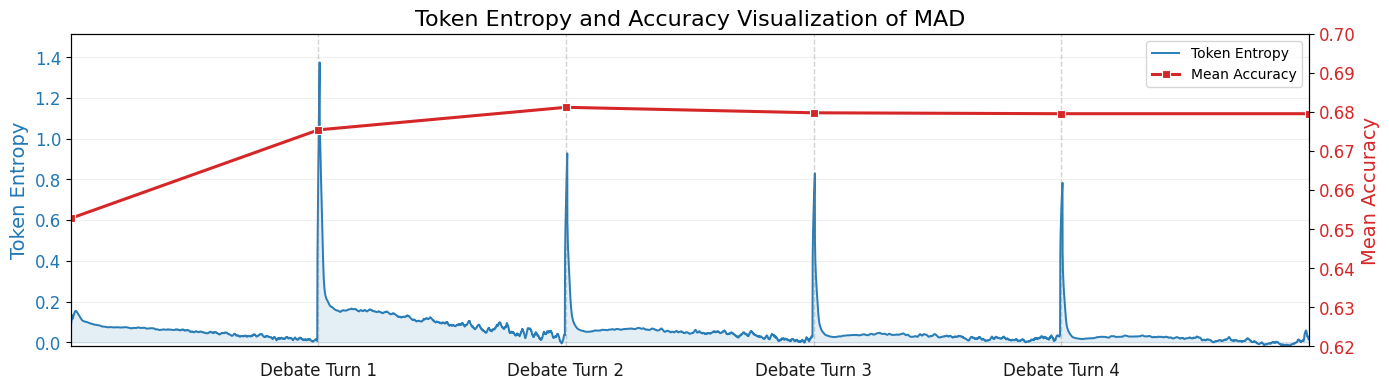
\includegraphics[width=0.9\linewidth]{fig/intro/entropy_acc.png}
    \caption{两个 \texttt{Qwen2.5-3B-Instruct} 模型参与多智能体辩论时的表现。随着准确率（红线）在各辩论轮次中上升，词元熵（蓝色阴影）也明显增大。}
    \label{fig:intro-entropy}
\end{figure}


\section{问题表述}


\subsection{多智能体辩论}

遵循标准 MAD 设置 \cite{du2023improving, park2025maporl}，我们将 MAD 表述为 $N$ 个智能体之间进行的 $T$ 步迭代生成过程，其中各智能体由 LLM 参数 $\{\pi_{\theta_i}\}_{i=1}^N$ 参数化。对从数据集中采样的问题 $x\sim\mathcal{D}$，存在真实答案 $y^*$。对于数学任务，推理过程可以多种多样，但答案在数值上通常唯一，而且往往可以通过与真实答案进行字符串匹配来精确验证。\footnote{本文略微复用记号，统一用 $y$ 表示完整回答和从中抽取的最终答案。} 在每一轮 $t \in \{0, \dots, T\}$，智能体 $i$ 以原始问题 $x$ 和不断变化的上下文 $c_{i,t}$ 为条件生成回答 $y_{i,t}\sim\pi_{\theta_i}(\cdot \mid x, c_{i,t})$；该上下文包含其他智能体的参考解答和额外的辩论指令。在初始轮 $t=0$，模型通常直接回答原问题 $x$，此时辅助上下文 $c_{i,0}$ 为空。形式上，智能体 $i$ 按如下方式自回归地生成含 $L$ 个词元的回答 $y_{i,t}$：
\begin{equation*}
   \pi_{\theta_i}(y_{i,t} \mid x, c_{i,t}) =  \prod_{l=1}^{L}\pi_{\theta_i}(y_l\mid x, c_{i,t}, y_{<l}).
\end{equation*}
回答通常会先给出中间推理步骤，再生成最终答案；在 OpenAI o1 和 DeepSeek-R1 等推理模型中，这些步骤可能由特殊标记 \texttt{</think>} 包围 \cite{openai_o1, guo2025deepseek}。尽管 MAD 提示存在多种信息组织方案 \cite{li2024improving, liu2024groupdebate, chen2024reconcile}，我们定义统一的上下文映射函数 $\Phi$，依据前几轮同伴回答的全局历史为每个智能体构造输入上下文：$c_{i,t} = \Phi_i(\{Y_k\}_{k=1}^{t-1}, \mathcal{G}, \mathcal{P})$。其中，$Y_k = \{y_{1, k}, \dots, y_{N, k}\}$ 表示所有智能体在第 $k$ 轮辩论中的回答；通信拓扑 $\mathcal{G}$ 决定智能体 $i$ 可以访问哪些同伴回答，例如全连接图或有向图；智能体角色提示 $\mathcal{P}$ 则决定每个智能体如何利用和处理同伴回答，例如直接拼接、引入额外 LLM 进行总结，或使用特定角色指令。在最终轮 $T$，汇总函数 $\Psi$ 从所有智能体的回答 $Y_T$ 中提炼系统预测 $\hat{y} = \Psi(Y_T)$；该函数可以是多数投票 \cite{du2023improving}、Elo \cite{zhang2025debate4math} 或 LLM-as-a-Judge \cite{zhu2023judgelm}。

本文关注单个智能体的推理能力，而不是为提高最终回答准确率而优化 MAD 工作流。因此，我们采用全连接通信图 $\mathcal{G}$，使每个智能体都能看到上一轮所有同伴的回答，同时不引入专门角色、总结模块或任务特定的通信规则。在实验和分析中，我们还去除了最终汇总函数 $\Psi$，使评估直接反映每个智能体辩论后回答 $y_{i,T}$ 的推理能力。该设置隔离了信息交换对单体推理行为的影响。


\subsection{可验证奖励强化学习}
可验证奖励强化学习（Reinforcement Learning with Verifiable Rewards，RLVR）已成为一种强大的范式：它利用基于规则、可验证的二值稀疏奖励信号，通过强化学习训练激发 LLM 的高阶复杂推理能力。近期工作建立在群组相对策略优化（Group Relative Policy Optimization，GRPO）\cite{shao2024deepseekmath} 之上；GRPO 是面向推理任务的专用强化学习算法，无需训练评论家模型。在标准单智能体设置中，对每个查询 $x$，LLM 策略 $\pi_\theta$ 采样一组 $G$ 个回答 $\{y_1, \dots, y_G\}$。对每个回答 $y_i$，奖励函数 $R(y_i, y^*)$ 评估其最终答案并给出二值奖励：答案正确时 $R=1$，否则 $R=0$。

GRPO 目标定义为：
\begin{equation}
\resizebox{0.96\columnwidth}{!}{$
\begin{aligned}
\mathcal{J}(\theta)
&= \mathbb{E}_{x \sim \mathcal{D}, \{y_i\}_{i=1}^G \sim \pi_\theta(\cdot \mid x)}
\Bigl[
\frac{1}{G}\sum_{i=1}^G \frac{1}{\lvert y_i\rvert}\sum_{j=1}^{\lvert y_i\rvert} \\
&\quad \Bigl(\min\Bigl(
r_{i,j}(\theta)A_{i,j},
\operatorname{clip}(r_{i,j},1-\epsilon,1+\epsilon)A_{i,j}
\Bigr) \\
&\qquad -\beta D_{\mathrm{KL}}(\pi_\theta \,\|\, \pi_{\mathrm{ref}})
\Bigr)
\Bigr].
\end{aligned}
$}
\end{equation}
其中，$r_{i,j} = \frac{\pi_\theta(y_{i,j}|x)}{\pi_{\theta_{old}}(y_{i,j}|x)}$ 表示词元级比率，$A_{i,j} = \frac{R_{i} - \text{mean}(\{R\}_{i=1}^G)}{\text{std}(\{R\}_{i=1}^G)}$ 表示组内归一化优势，$\beta$ 控制 KL 散度惩罚。这种无评论家的方法能够有效稳定 LLM 推理训练，已广泛用于数学、代码和智能体训练任务 \cite{yu2025dapo,wei2025swe,jin2025search}。如第 \ref{subsec:MAD_POMDP} 节所述，本文将 MAD 视为可学习的多智能体多步决策过程，并以轮次级可验证奖励优化每个策略 $\pi_{\theta_i}$，从而把 GRPO 扩展到多智能体辩论。


\section{MAD 中的不确定性机制}
\label{sec:theory}


本节从不确定性分解的视角分析多智能体辩论（MAD）的动态。我们将贝叶斯表述作为概念框架，并明确区分潜在信念变量、答案层面的诊断代理以及训练时优化代理。第 \ref{subsec: iterative_bayes} 节将辩论形式化为迭代贝叶斯信念更新过程，其中同伴回答充当带噪证据。第 \ref{subsec: system_uncertainty} 节用答案层面的预测分布将这一观点具体化，并将系统级不确定性分解为认知分量与偶然分量。第 \ref{subsec:agent_uncertainty} 节进一步研究辩论上下文变化时单个智能体的不确定性，并解释异构同伴何时能够提供额外的认知增益。


\subsection{MAD 的迭代贝叶斯信念更新}\label{subsec: iterative_bayes} 
近期研究将 LLM 视为隐式贝叶斯推断过程 \cite{jayasekera2025variational, xie2021explanation, choi2025debate}。受此启发，我们把智能体 $i$ 的回答生成形式化为分层采样过程，以便从观测到的文本回答 $y_{i,t}$ 中分离出潜在信念 $\varphi_{i,t}$。潜在信念变量 $\varphi_{i,t}$ 表示智能体在辩论上下文 $c_{i,t}$ 下对解法假设的隐式分布，包括相关定理、中间推理方案和候选最终答案\footnote{为简化记号，下文在上下文清楚时省略 $\varphi_{i,t}$ 中的轮次下标 $t$。}。它可以反映智能体当前对问题的理解，例如数学定理、分析方法和解题逻辑。
随后，LLM 在词表空间中进行自回归采样，得到观测文本回答 $y_{i,t}$；该过程可视为由潜在信念 $\varphi_i$ 驱动，即 $y_{i,t} \sim p(y \mid \varphi_{i})$。由于 MAD 推理期间 LLM 参数 $\theta_i$ 保持冻结，对潜在信念积分后可得回答的后验预测分布：
\begin{equation*}
 p(y_{i,t} \mid x,c_{i,t}) = \int p(y_{i,t} \mid \varphi_{i})\,p(\varphi_{i} \mid x,c_{i,t})\,d\varphi_{i}.
\end{equation*}
因此，从概念上看，MAD 通过多轮辩论更新回答的过程可以理解为迭代贝叶斯信念更新。通过加入额外的参考解答来改变轮间上下文 $c_{i,t}$，智能体的潜在信念 $p(\varphi_i\mid x,c_{i,t})$ 被隐式更新，进而改变后验预测分布 $p(y_{i,t}\mid x,c_{i,t})$，并可能改变最终答案。例如，相较于首轮初始回答 $y_{i,0}$，第 $t$ 轮更新后的信念可建模为对潜变量进行如下贝叶斯更新：
\begin{equation}\label{eq:bayes_belief}
 p(\varphi_{i} \mid x,c_{i,t})
\ \propto\
p(c_{i,t}\mid \varphi_{i},x)\;p(\varphi_{i} \mid x),
\end{equation}
其中，$p(c_{i,t}\mid \varphi_i,x)$ 表示在上下文 $c_{i,t}$ 下，给定智能体潜在信念状态时同伴参考解答的隐式似然。直观而言，有效的辩论上下文可以使智能体的后验信念移向真实答案，从而借助更优的后验 $p(y_{i,t}\mid x,c_{i,t})$ 提高预测准确率。


不同于选项有限的选择题，数学推理问题的答案空间往往可能是无限的。考虑到真实答案在等价关系意义下通常唯一，我们可以用第 $t$ 轮智能体 $i$ 的二值正确性事件 $h_{i,t} := \mathbf{1}[y_{i,t}\in \mathcal{Y}^*]\in\{0,1\}$ 简化信念空间，其中 $\mathcal{Y}^*\subseteq\mathcal{Y}$ 表示与真实答案等价的回答集合。
相应地，对正确性的预测信念为
\begin{equation*}
p(h_{i,t}=1\mid x,c_{i,t})
=
\sum_{y\in \mathcal{Y}^*} p(y_{i,t}=y\mid x,c_{i,t}).
\end{equation*}
为简化记号，我们省略智能体下标，并用 $c_t$ 表示某个固定智能体接收到的辩论上下文。关于第 $t$ 轮智能体 $i$ 的回答正确性，有如下引理：
\begin{lemma}[带噪证据的对数优势更新]\label{lem:log_odds}
给定输入问题 $x$，假设初始上下文为空，并且辩论上下文 $c_t$ 有效，即 $p(c_t\mid x)>0$，则辩论后二值假设 $h\in\{0,1\}$ 的对数优势可写为
{\small
\begin{equation*}
    \log \frac{p(h=1 \mid x,c_t)}{p(h=0 \mid x,c_t)}
=
\log \frac{p(h=1 \mid x)}{p(h=0 \mid x)}
+
\log \frac{p(c_t \mid h=1, x)}{p(c_t \mid h=0, x)}.
\end{equation*}
}
\end{lemma}

引理~\ref{lem:log_odds} 可由贝叶斯法则直接证明，证明见附录~\ref{app:proof_lemma1}。


加性项 $\log \frac{p(c_t \mid h=1, x)}{p(c_t \mid h=0, x)}$ 是由辩论上下文引起的\textit{对数贝叶斯因子}。正值表示上下文提供了支持正确性的证据，可能促成从错误到正确（$W\to C$）的转变；负值则表示证据具有误导性或未被妥善利用，可能使后验信念偏离真实答案，并促成从正确到错误（$C\to W$）的转变。它为既有 MAD 研究中观察到的辩论停滞与答案翻转 \cite{choi2025debate, wynn2025talk, yao2025peacemaker} 提供了贝叶斯解释。这一观察说明，MAD 并不能保证单调地利用同伴提供的正确线索：即使同伴解答包含有用信息，智能体的内部信念仍可能被推向错误回答。


\begin{figure*}[t]
    \centering
    \begin{subfigure}{0.32\linewidth}
        \centering
        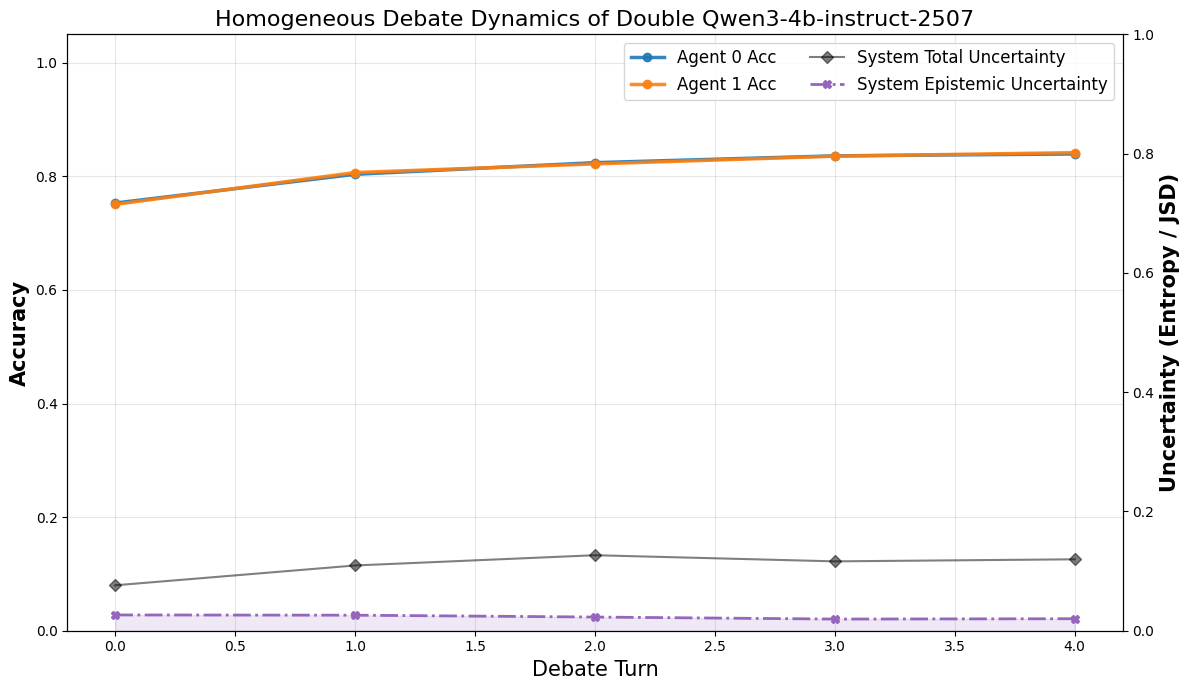
\includegraphics[width=\linewidth]{fig/main_uncertainty/double_2507.png}
        \caption{成功的同构 MAD}
    \end{subfigure}
    \begin{subfigure}{0.32\linewidth}
        \centering
        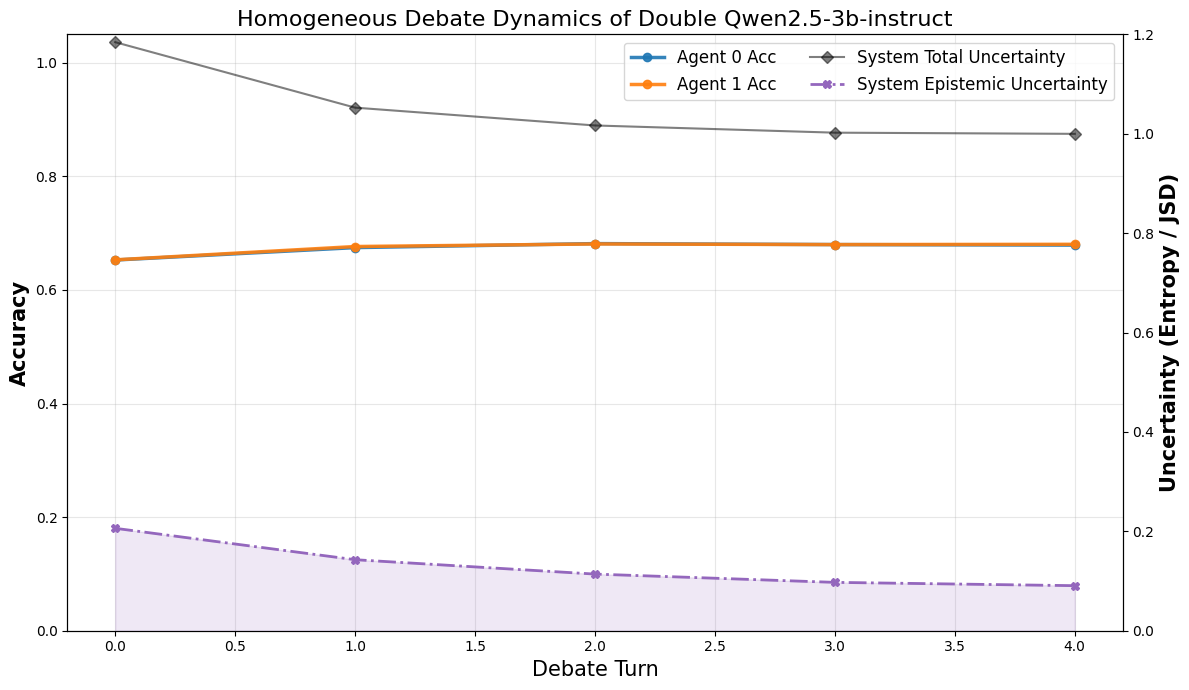
\includegraphics[width=\linewidth]{fig/main_uncertainty/double_2.5-3.png}
        \caption{中性的同构 MAD}
    \end{subfigure}
    \begin{subfigure}{0.32\linewidth}
        \centering
        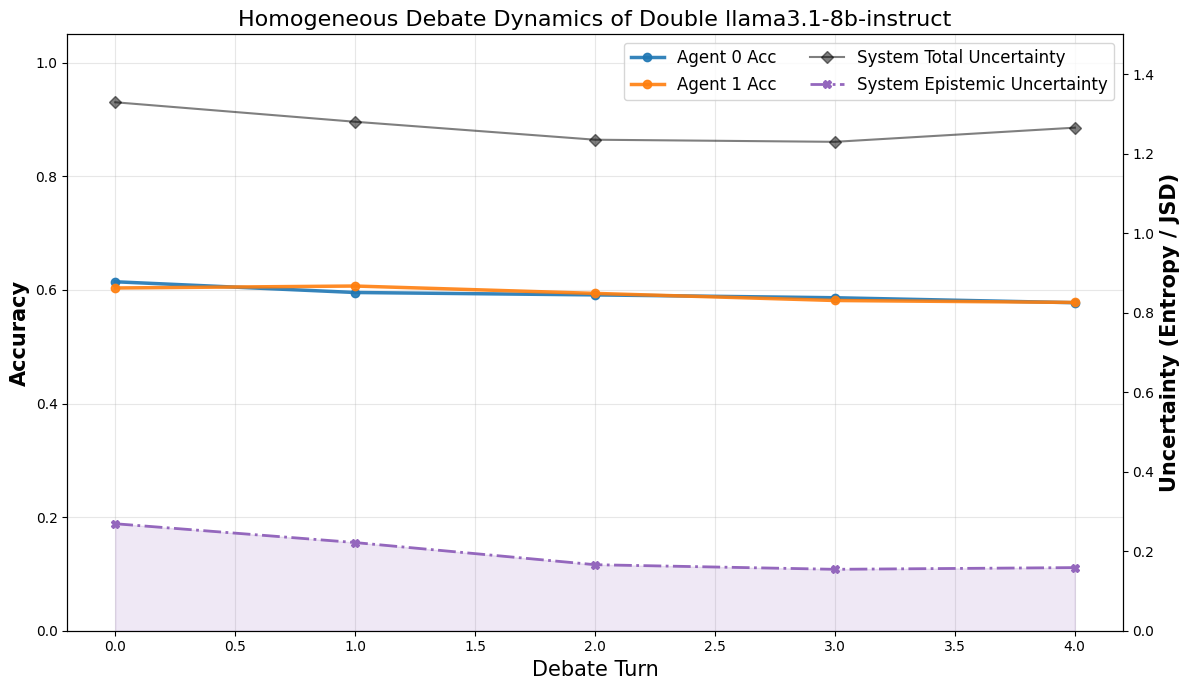
\includegraphics[width=\linewidth]{fig/main_uncertainty/double-llama8.png}
        \caption{失败的同构 MAD}
    \end{subfigure}

    \vspace{0.5em}

    \begin{subfigure}{0.32\linewidth}
        \centering
        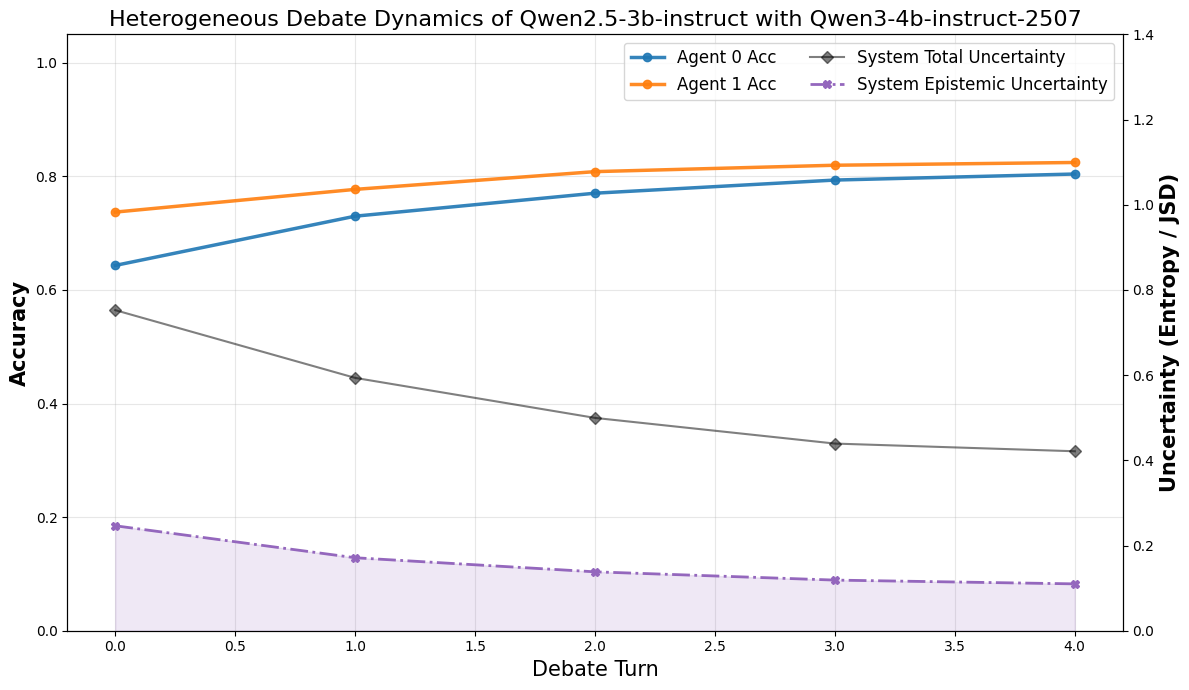
\includegraphics[width=\linewidth]{fig/main_uncertainty/hetero-2.5_2507.png}
        \caption{成功的异构 MAD}
    \end{subfigure}
    \begin{subfigure}{0.32\linewidth}
        \centering
        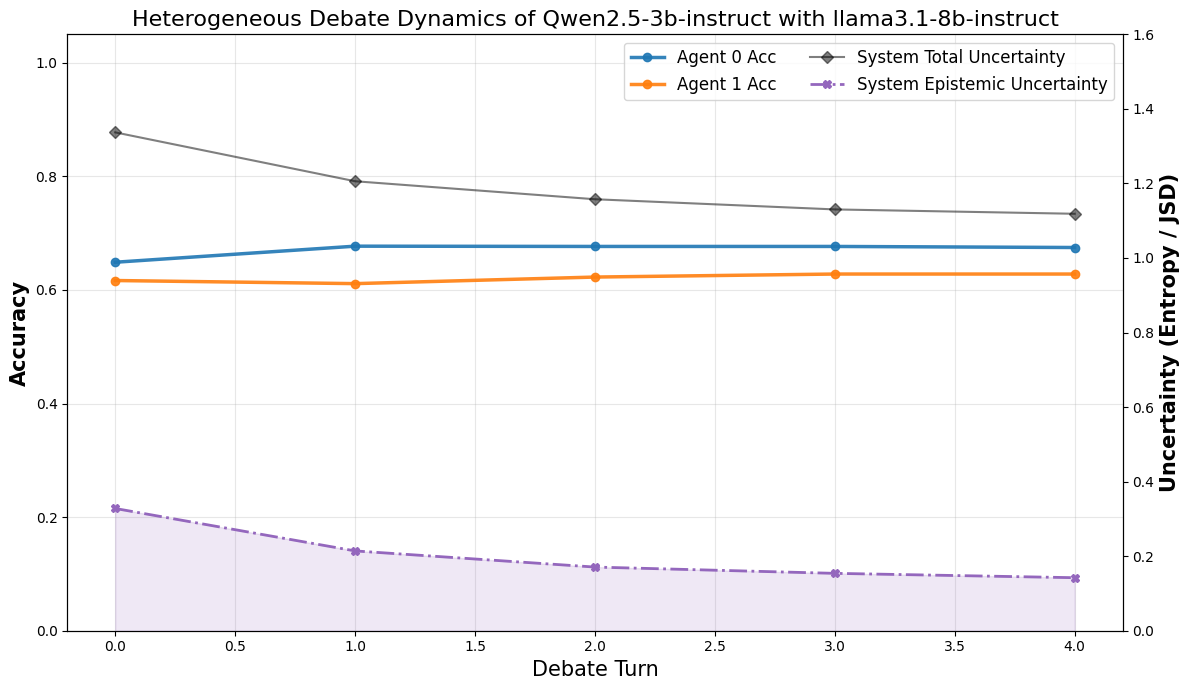
\includegraphics[width=\linewidth]{fig/main_uncertainty/hetero-2.5_llama8.png}
        \caption{中性的异构 MAD}
    \end{subfigure}
    \begin{subfigure}{0.32\linewidth}
        \centering
        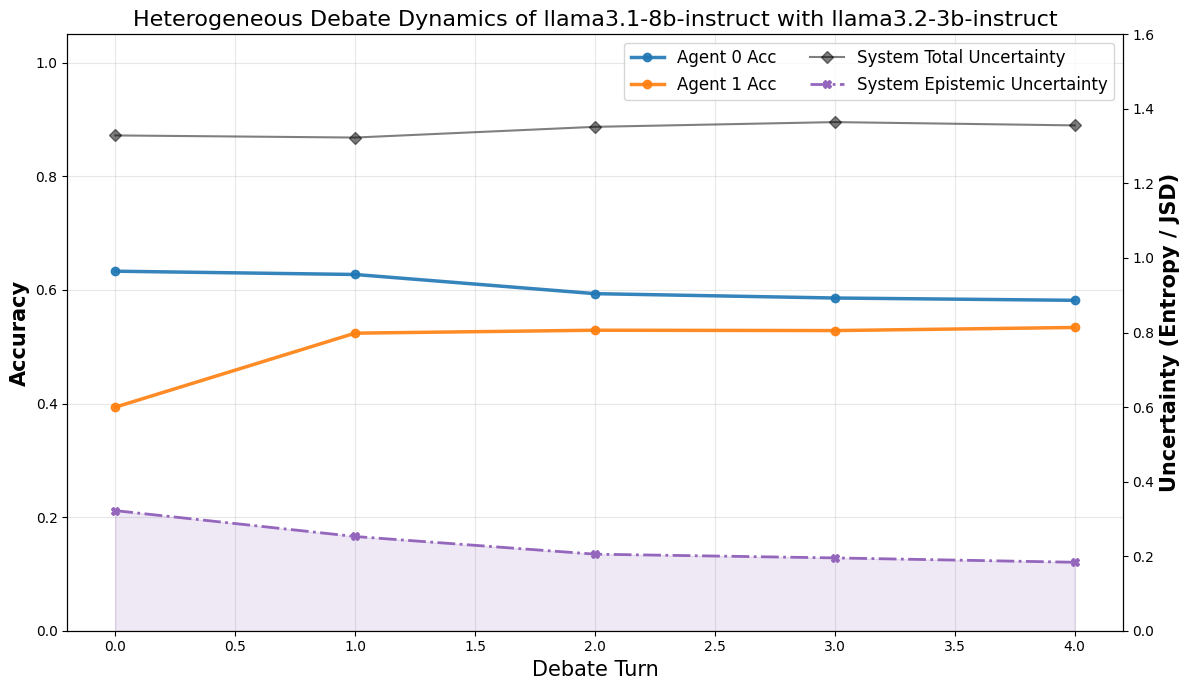
\includegraphics[width=\linewidth]{fig/main_uncertainty/hetero-llama8-llama3.png}
        \caption{失败的异构 MAD}
    \end{subfigure}

    \caption{MAD 中的不确定性分解概览。紫色虚线区域表示系统认知不确定性，灰线表示总不确定性；总不确定性与 Sys-EU 之间的差对应 Sys-AU。蓝线和橙线表示测试数据集上的准确率。
    \textbf{上排：}同构多智能体辩论。
    \textbf{下排：}异构多智能体辩论。}
    \label{fig:intro-total}
\end{figure*}



\subsection{MAD 中的系统级不确定性权衡}\label{subsec: system_uncertainty}

量化大模型的不确定性对于理解回答的可靠性至关重要。然而，由于 LLM 参数规模庞大、生成空间维度极高，基于深度贝叶斯网络或 dropout 推断的传统不确定性估计方法 \cite{lakshminarayanan2017simple, li2017dropout} 并不适用于基于 LLM 的推理。此外，对大型 LLM 而言，隐式潜在信念状态 $\varphi_i$ 在计算上同样不可处理 \cite{abbasi2024believe,jayasekera2025variational}。为克服这些限制，我们考虑基于答案层面的预测分布，对 MAD 系统的不确定性进行量化和分解。



核心直觉是，可以将 MAD 系统视为一组预测专家的集成。给定同一个问题 $x$ 和辩论上下文 $C_t=\{c_{i,t}\}_{i=1}^N$，每个智能体都会诱导一个答案层面的预测分布 $p_{i,t}(y)$。实践中，我们在相同的 $(x,c_{i,t})$ 条件下从智能体 $i$ 采样 $G$ 个回答并抽取其最终答案，以估计 $p_{i,t}(y)$。该经验分布刻画了当前辩论上下文下智能体最终答案预测的稳定或分散程度。我们不把这些样本视为从联合贝叶斯模型中精确抽取的后验样本，而是采用专家集成代理，并将系统级预测分布定义为 $p_{\mathrm{sys},t}:=\frac{1}{N}\sum_{i=1}^N p_{i,t}$。

在一个温和假设下，这一集成代理也与贝叶斯信念更新一致：每个智能体的分布 $p_i(y)$ 可视为与隐式采样相对应的一个专家，跨专家平均因而近似于贝叶斯模型平均。因此，混合分布 $p_{\mathrm{sys},t}$ 可以解释为近似后验预测分布。我们将总不确定性（TU）量化为集体答案层面预测分布的熵。该混合熵具有经典全熵定律 \cite{lakshminarayanan2017simple} 在答案层面的对应形式，可分解为系统认知不确定性（Sys-EU）与系统偶然不确定性（Sys-AU）：


\begin{proposition}[答案层面的系统不确定性分解]\label{prop:sys_decomp}
设 $\{p_{i,t}\}_{i=1}^N$ 表示第 $t$ 轮各智能体在答案层面的预测分布，其混合分布为
$p_{\mathrm{sys},t}=\frac{1}{N}\sum_{i=1}^N p_{i,t}$。则答案层面的总不确定性可分解为
\begin{align}
\underbrace{H(p_{\mathrm{sys},t})}_{\mathrm{TU}(t)}= 
\underbrace{\mathrm{JSD}(p_{1,t},\ldots,p_{N,t})}_{\mathrm{Sys\mbox{-}EU}}
+
\underbrace{\frac{1}{N}\sum_{i=1}^N H(p_{i,t})}_{\mathrm{Sys\mbox{-}AU}}.
\label{eq:sys_decomp}
\end{align}
\end{proposition}


命题~\ref{prop:sys_decomp} 可由广义 Jensen-Shannon 散度的定义证明，证明见附录~\ref{app:proof_prop2}。对答案层面的混合分布而言，该恒等式是精确的；将其解释为认知不确定性和偶然不确定性则是一种操作性定义。具体而言，Sys-EU 衡量智能体答案分布之间的分歧，因此作为可约减的智能体间不确定性的代理；Sys-AU 衡量单个智能体答案分布的平均熵，因此作为回答不稳定性的代理。该分解并不假设 Sys-EU 与 Sys-AU 在各辩论轮次之间统计独立，而是把答案层面的熵拆分为两个可加分量。在确定性数学推理任务中，Sys-AU 主要并非源自标签固有歧义，而是来自生成随机性、长上下文扰动以及对同伴回答的带噪利用 \cite{feng2025rethinking, ling2024uncertainty}。


为检验这一操作性分解能否捕捉辩论动态，我们在 MATH~\cite{hendrycks2021measuring} 数据集的一个子集上评估同构和异构 MAD 配置，其中智能体数 $N=2$，辩论轮数 $T=5$，每个提示采样 $G=5$ 条轨迹（详细设置见附录~\ref{app:sys_uncertainty_decomposition}）。如图~\ref{fig:intro-total} 所示，在所有设置中，$\mathrm{Sys\mbox{-}EU}$ 通常随辩论轮次减少。这表明 MAD 倾向于缩小智能体间分歧并推动智能体达成共识，尽管这种共识未必正确。

关键在于，不同配置之间的性能差异主要可由降低 $\mathrm{Sys\mbox{-}EU}$ 与控制 $\mathrm{Sys\mbox{-}AU}$ 之间的平衡来解释。成功的辩论会使 $\mathrm{Sys\mbox{-}AU}$ 保持较低或持续下降；失败案例中的 $\mathrm{Sys\mbox{-}AU}$ 则居高不下或继续上升，抵消了减少分歧带来的收益。这一权衡也说明了智能体异构性何时有利。异构配对的初始 $\mathrm{Sys\mbox{-}EU}$ 通常高于同构配对，表明其认知差距更大、信息交换潜力更高。然而，只有当接收方能够可靠处理同伴论证，且不会引入过多生成不稳定性时，这种认知潜力才会转化为收益。附录~\ref{subsec:flip_dynamics} 的翻转率分析支持这一观点：跨模型族配对能形成较大的认知差距，却也可能引入额外不稳定性；同一模型族内部的规模异构或生成异构往往能取得更好的平衡。实践中，翻转率较低的强模型可充当稳定锚点，而较弱一方必须保有足够的指令遵循能力，才能综合同伴推理，而不是来回摇摆或盲目从众。

\subsection{异构 MAD 的认知优势}\label{subsec:agent_uncertainty}
上一节~\ref{subsec: system_uncertainty} 的系统级不确定性分析表明，辩论准确率同时受到认知增益与偶然成本的影响，但这还不足以解释某条具体的同伴回答何时会为单个智能体提供有用信息。因此，我们分析单个智能体在接收同构与异构同伴消息时的不确定性变化。关键在于区分单纯分歧和有用分歧：较高的系统级分歧意味着存在可用的认知潜力，但只有当同伴消息针对该智能体的潜在解法信念提供了非冗余证据时，智能体才能从中获益。


遵循第~\ref{subsec: iterative_bayes} 节的贝叶斯观点，设 $\varphi$ 表示智能体在当前问题 $x$ 和上下文 $c$ 下对解法假设的潜在信念。我们将额外同伴消息 $m$ 提供的认知增益定义为
\[
G_{\mathrm{epi}}(m \mid x,c) := I(\varphi; m \mid x,c).
\]
该量衡量同伴消息为智能体潜在信念状态提供了多少信息。在 MAD 中，较高的认知增益对应于这样的证据：它能引入有用的解法假设、纠正误导性推理路径，或帮助智能体区分相互竞争的答案。从操作角度看，对某智能体反复采样可以近似其当前信念下可到达的答案支撑，类似于 \texttt{pass@K} 视角。当同伴的采样回答覆盖了接收方尚未覆盖的解法模式时，该同伴便是有用的。
下面我们形式化说明同构辩论为何通常只能有限地改善单个智能体。由于采样随机性，同构同伴可能生成不同回答，但它们的答案支撑与推理偏差往往高度重叠。因此，在观察到一条同构消息后，另一条同构消息往往只能提供有限的额外信息。
\begin{assumption}[同构信息饱和]\label{ass:homo_saturation}
给定当前问题 $x$ 和上下文 $c$，设 $m_{\mathrm{homo}}$ 与 $m'_{\mathrm{homo}}$ 是来自同构同伴的两条独立消息。在以一条同构消息为条件后，另一条同构消息所提供的额外条件信息有如下上界：
\[
I(\varphi; m'_{\mathrm{homo}} \mid x,c,m_{\mathrm{homo}})
\le
\epsilon_{\mathrm{homo}}.
\]
\end{assumption}


该假设并非对所有智能体作出的普遍断言，而是针对一种常见情形的诊断条件：同模型样本的边际新颖性逐渐递减。它刻画了“支撑重叠”这一直觉：同构智能体在表面上可能意见不同，但它们往往探索解空间中的相似区域。因此，同构辩论能够减少分歧并促使智能体达成共识，却未必会显著扩展接收方对有效解法的支撑 \cite{choi2025debate, zhang2025if, wynn2025talk}。


\begin{theorem}[互补性条件下的异构认知优势]\label{thm:hetero_gain}
假设~\ref{ass:homo_saturation} 成立。设 $m_{\mathrm{hetero}}$ 是来自异构同伴的消息。若该异构消息提供的互补证据超过同构饱和水平，即
\[
I(\varphi; m_{\mathrm{hetero}} \mid x,c,m_{\mathrm{homo}})
\ge
\epsilon_{\mathrm{homo}} + \Delta
\]
对某个 $\Delta \ge 0$ 成立，则用该异构消息替换第二条同构消息，会使认知信息总量至少增加 $\Delta$：
\[
\begin{aligned}
&I(\varphi; m_{\mathrm{homo}},m_{\mathrm{hetero}} \mid x,c) \\
&\quad - I(\varphi; m_{\mathrm{homo}},m'_{\mathrm{homo}} \mid x,c)
\ge \Delta.
\end{aligned}
\]
\end{theorem}

定理~\ref{thm:hetero_gain} 可由条件互信息的链式法则证明，证明见附录~\ref{app:proof_theo3}。该定理说明，异构 MAD 的优势来自条件新颖性，而不是模型多样性本身。异构智能体可以提供超出同构同伴推断范围的互补证据，从而扩展接收方对有效解法的支撑，并创造更大的由错转对潜力。这也解释了同构辩论为何经常停滞：当另一条同模型消息的条件新颖性很小时，分歧减少主要反映的是冗余的共识形成，而非真正的信念扩展 \cite{wynn2025talk}。


然而，该定理刻画的是认知潜力，而非有保证的准确率提升。如第~\ref{subsec: system_uncertainty} 节所示，只有当接收方能够在偶然成本受控的情况下吸收互补证据时，这种潜力才会转化为性能收益。这也解释了异构 MAD 的失败模式：例如，图~\ref{fig:intro-total} 中基于 Llama 的失败案例仍表现出不可忽略的分歧下降，但由此引发的回答不稳定性使 $\mathrm{Sys\mbox{-}AU}$ 居高不下，足以抵消认知收益。因此，目标不应只是最大化互补认知增益 $\Delta$，而应在控制偶然成本的同时实现这一增益。这一权衡引出了后续的\emph{训练时优化代理}：它们鼓励智能体吸收有用的异构证据，同时抑制辩论中的不稳定性。

   

\section{面向 MAD 的不确定性引导 MARL}
\label{sec:method}

根据第 \ref{sec:theory} 节的分析，有效的 MAD 需要在实现同伴所提供的互补认知信息的同时，控制辩论引入的偶然不稳定性。因此，我们将 MAD 建模为 MARL 问题，以改善智能体在辩论中使用同伴信息的方式。我们的方法称为\textbf{不确定性引导的多智能体辩论（Uncertainty-Guided Multi-Agent Debate，UMAD）强化学习}，它利用回答的可验证奖励来优化智能体策略，鼓励智能体吸收有用的同伴证据，同时抑制不稳定生成。


\subsection{将 MAD 建模为 Dec-POMDP} \label{subsec:MAD_POMDP}

受多个 LLM 协作训练的近期工作 \cite{park2025maporl,liao2025marft, wan2025rema} 启发，我们将多智能体辩论强化学习表述为分散式部分可观测马尔可夫决策过程（Dec-POMDP）\cite{oliehoek2016concise}，其由元组 $\langle \mathcal{N}, \mathcal{S}, \mathcal{A}, P, R, \Omega, \mathcal{O}, \gamma \rangle$ 定义。

具体而言，在每一轮 $t$，每个智能体 $i \in \{1, \dots, N\}$ 观测局部上下文 $o_{i,t}=x\oplus c_{i,t}$，它由原始查询和基于先前同伴回答构造的辩论上下文组成。LLM $i$ 生成的回答序列记为 $a_{i,t}$，它是智能体 $i$ 在步骤 $t$ 的动作，包含中间推理步骤和最终答案。为促进协作改进，我们采用稠密团队奖励 $R_t = \sum_i r(a_{i,t}, y^*)$，其中每个个体奖励都通过验证抽取出的最终答案来计算。考虑到训练 LLM 的复杂性和高计算需求，我们采用独立学习范式作为算法骨干，使每个智能体最大化预期联合回报。然而，在 MAD 中，标准独立学习往往面临非平稳性和信用分配粗糙的问题。我们使用一种双管齐下的不确定性引导机制解决这些问题。


\subsection{不确定性引导的优化机制} \label{sec:mechanisms}

基于第 \ref{sec:theory} 节识别出的不确定性权衡，我们引入两个易于计算的训练时代理，在策略优化期间促进认知信息利用并降低偶然不稳定性。




\textbf{偶然不确定性感知优势。}辩论中的智能体往往表现出置信度失准，体现为“顽固幻觉”或“犹豫推理”。为调节偶然噪声，我们采用置信度感知的优势塑形机制。受 UCAS~\cite{xie2025unlocking} 启发，我们用词元级负对数概率作为生成不确定性的实用代理。对每个回答 $y_{i,t}$，首先计算词元平均负对数概率：
\begin{equation*}
\hat{\mathcal{U}}_{i,t}
=
-\frac{1}{|y_{i,t}|}
\sum_{j=1}^{|y_{i,t}|}
\log \pi_{\theta_i}(y_{i,t,j}\mid x,c_{i,t},y_{i,t,<j}),
\end{equation*}
它可以在 GRPO 采样组内标准化为 $
\bar{\mathcal{U}}_{i,t}
=
\frac{\hat{\mathcal{U}}_{i,t}-\mu_{\mathcal{G}}}{\sigma_{\mathcal{G}}+\epsilon}.$ 随后按如下方式调节标准优势 $A_{i,t}$：
\begin{equation}
A^{\mathrm{au}}_{i,t}
=
W(\bar{\mathcal{U}}_{i,t}) A_{i,t},
\end{equation}
其中，依赖不确定性的权重定义为
$W(\bar{\mathcal{U}}_{i,t})
=
\exp(-\alpha_{\mathrm{au}}\bar{\mathcal{U}}_{i,t}),
$，$\alpha_{\mathrm{au}}$ 为超参数。该词元级信号是回答不稳定性的实用代理，而不是语义偶然不确定性的精确估计。此塑形方法降低高不确定性回答的权重，从而减轻长上下文扰动或异构同伴上下文所导致的带噪生成的影响。





\textbf{认知影响内在奖励。}为促进认知信息增益 $G_{\text{epi}}$，有效辩论要求智能体不仅自身正确，还要对同伴有用。其核心直觉是，同一条同伴消息对潜在信念不同的智能体可能产生不同影响。因此，除正确性奖励外，我们还需要激励那些更容易被其他智能体有效利用的回答。我们引入内在奖励 $r^{\text{eu}}_{i,t}$，量化对同伴可观测的正向影响：
\begin{equation} r^{\text{eu}}_{i,t} = \frac{\eta}{N-1} \sum_{j \neq i} \Delta R_{\text{peer}}(j, t+1), \end{equation} 
其中，$\Delta R_{\text{peer}}$ 表示在加入智能体 $i$ 的参考解答后，GRPO 多条采样轨迹的平均正确率提升。虽然该机制不直接计算互信息，但它奖励那些能够提高同伴下一轮平均正确率的回答，因而可作为认知影响的可观测代理。


\section{实验}
\label{sec:experiments}

\subsection{实验设置}
\textbf{辩论配置。}
对于同构辩论，我们以两个 \texttt{Qwen2.5-3B-Instruct} 智能体分别作为 $A0$ 和 $A1$，构成一个指令遵循与数学推理能力可靠、较为稳定的同模型设置。为在保持指令遵循能力相近的同时构造具有模型多样性的异构辩论系统，我们从 Qwen 系列中选择两个代际不同的模型：\texttt{Qwen2.5-3B-Instruct}（$A0$）和 \texttt{Qwen3-4B-Instruct-2507}（$A1$）\cite{yang2024qwen2,yang2025qwen3}。

\textbf{数据集。}我们在含 7,500 个训练样本的 MATH 数据集 \cite{hendrycks2021measuring} 上训练智能体，采用 $T_{train}=2$ 的两轮辩论训练协议。该设置用于评估：从短程局部交互中学得的辩论策略，能否泛化到更长的推理时辩论，而无需昂贵的长时域训练。推理时，我们将辩论延长至 $T_{test}=5$ 轮，以评估其抵抗模式崩溃的稳健性与泛化能力。我们在从 MATH 中抽取 500 个样本构成的 MATH500 数据集上评估分布内性能，并在从小学数学（GSM8K \cite{cobbe2021training}）到奥林匹克竞赛级别（AMC2023、AIME24、AIME25 \cite{amc2023,aops_aime_2024, aops_aime_2025}）的一系列分布外任务上评估泛化能力。



\textbf{基线。}
主表将 UMAD 与零样本 MAD 和标准 IPPO 进行比较。零样本 MAD 是推理时辩论基线，标准 IPPO 则是不含不确定性引导的多智能体强化学习基线。在附录~\ref{app:supply_au_eu} 中，我们进一步加入强力的单体 GRPO 配对基线：每个模型分别采用标准 GRPO 设置独立微调 15 个 epoch 直至收敛，再在相同辩论协议下评估。该基线使用的单体训练量多于 UMAD，用于检验收益是否仅仅来自更强的单个模型。除非另有说明，所有主要结果均在五个评估随机种子上取平均，报告的 $\pm$ 数值表示不同种子之间的评估波动。



\begin{table*}[t]
\centering
\caption{初始回答（$T=1$）与辩论回答（$T=2, 5$）中单个智能体准确率的比较。我们报告使用 \texttt{Qwen2.5-3B-Instruct} 和 \texttt{Qwen3-4B-Instruct-2507} 的同构及异构 MAD 设置下的 \texttt{pass@1} 结果。浅蓝色 \capbox{MBlue!25}{+ 增益} 和浅粉色 \capbox{MPink!25}{- 损失} 表示性能变化。单元格颜色相对于同一轮次（$T$）对应的\texttt{零样本}基线确定。粗体表示 $T=5$ 时\texttt{零样本}、\texttt{IPPO} 和 \texttt{UMAD} 中的最佳表现。}
\label{tab:main_results}
\small
\setlength{\tabcolsep}{3.5pt} 
\resizebox{0.95\textwidth}{!}{
\begin{tabular}{l|l|cc|cc|cc|cc|cc|cc}
\toprule
\multirow{2}{*}{\textbf{设置}} & \multirow{2}{*}{\textbf{方法（轮次）}} & \multicolumn{2}{c|}{\textbf{GSM8K}} & \multicolumn{2}{c|}{\textbf{MATH500}} & \multicolumn{2}{c|}{\textbf{AMC23}} & \multicolumn{2}{c|}{\textbf{AIME24}} & \multicolumn{2}{c|}{\textbf{AIME25}} & \multicolumn{2}{c}{\textbf{平均}} \\
 & & \textbf{A0} & \textbf{A1} & \textbf{A0} & \textbf{A1} & \textbf{A0} & \textbf{A1} & \textbf{A0} & \textbf{A1} & \textbf{A0} & \textbf{A1} & \textbf{A0} & \textbf{A1} \\
\midrule
\multirow{9}{*}{\shortstack[l]{同构\\MAD}} 
& \bgbase{Zero-Shot ($T=1$)} & \bgbase{$\sd{83.3}{0.4}$} & \bgbase{$\sd{83.3}{0.4}$} & \bgbase{$\sd{61.0}{0.5}$} & \bgbase{$\sd{61.0}{0.5}$} & \bgbase{$\sd{35.0}{1.2}$} & \bgbase{$\sd{45.0}{1.1}$} & \bgbase{$\sd{3.3}{0.0}$} & \bgbase{$\sd{0.0}{0.0}$} & \bgbase{$\sd{2.0}{1.8}$} & \bgbase{$\sd{2.0}{1.8}$} & \bgbase{$\sd{36.9}{0.4}$} & \bgbase{$\sd{38.3}{0.4}$} \\
& IPPO ($T=1$) & \bg[10]{$\sd{83.4}{0.3}$} & \bged[15]{$\sd{82.3}{0.4}$} & \bg[35]{$\sd{65.2}{0.5}$} & \bg[15]{$\sd{62.2}{0.6}$} & \bg[50]{$\sd{45.0}{1.2}$} & \bg[0]{$\sd{45.0}{1.1}$} & \bg[0]{$\sd{3.3}{0.4}$} & \bg[5]{$\sd{1.5}{0.3}$} & \bg[5]{$\sd{2.7}{0.4}$} & \bg[5]{$\sd{2.7}{0.4}$} & \bg[25]{$\sd{39.9}{0.4}$} & \bg[5]{$\sd{38.7}{0.5}$} \\
& UMAD ($T=1$) & \bged[10]{$\sd{82.6}{0.4}$} & \bg[5]{$\sd{83.7}{0.3}$} & \bg[15]{$\sd{62.4}{0.5}$} & \bg[20]{$\sd{63.4}{0.4}$} & \bg[40]{$\sd{42.5}{1.4}$} & \bged[30]{$\sd{37.5}{1.6}$} & \bg[5]{$\sd{4.0}{0.5}$} & \bg[10]{$\sd{2.0}{0.4}$} & \bg[5]{$\sd{3.3}{0.6}$} & \bg[5]{$\sd{3.3}{0.5}$} & \bg[15]{$\sd{39.0}{0.5}$} & \bged[5]{$\sd{38.0}{0.6}$} \\
\cmidrule(l{0pt}r{0pt}){2-14}
& \bgbase{Zero-Shot ($T=2$)} & \bgbase{$\sd{83.4}{0.3}$} & \bgbase{$\sd{84.1}{0.4}$} & \bgbase{$\sd{63.0}{0.5}$} & \bgbase{$\sd{64.6}{0.6}$} & \bgbase{$\sd{30.0}{1.3}$} & \bgbase{$\sd{40.0}{1.2}$} & \bgbase{$\sd{3.3}{0.0}$} & \bgbase{$\sd{2.0}{1.8}$} & \bgbase{$\sd{6.7}{0.0}$} & \bgbase{$\sd{2.0}{1.8}$} & \bgbase{$\sd{37.3}{0.0}$} & \bgbase{$\sd{38.5}{0.6}$}\\
& IPPO ($T=2$) & \bg[0]{$\sd{83.4}{0.2}$} & \bged[15]{$\sd{83.3}{0.3}$} & \bg[25]{$\sd{65.8}{0.4}$} & \bged[10]{$\sd{64.2}{0.5}$} & \bg[55]{$\sd{42.5}{1.3}$} & \bg[35]{$\sd{47.5}{1.1}$} & \bg[10]{$\sd{4.0}{0.6}$} & \bg[5]{$\sd{2.7}{0.4}$} & \bg[5]{$\sd{7.3}{0.5}$} & \bg[5]{$\sd{3.3}{0.4}$} & \bg[25]{$\sd{40.6}{0.4}$} & \bg[15]{$\sd{40.2}{0.4}$} \\
& UMAD ($T=2$) & \bg[10]{$\sd{83.9}{0.3}$} & \bg[0]{$\sd{84.1}{0.2}$} & \bg[10]{$\sd{63.4}{0.4}$} & \bged[15]{$\sd{63.8}{0.5}$} & \bg[60]{$\sd{47.5}{1.2}$} & \bg[45]{$\sd{50.0}{1.0}$} & \bg[10]{$\sd{4.7}{0.7}$} & \bg[5]{$\sd{3.3}{0.5}$} & \bg[10]{$\sd{8.0}{0.8}$} & \bg[10]{$\sd{4.0}{0.6}$} & \bg[35]{$\sd{41.5}{0.4}$} & \bg[20]{$\sd{41.0}{0.5}$}\\
\cmidrule(l{0pt}r{0pt}){2-14}
& \bgbase{Zero-Shot ($T=5$)} & \bgbase{$\sd{83.4}{0.4}$} & \bgbase{$\sdb{84.6}{0.3}$} & \bgbase{$\sd{64.4}{0.5}$} & \bgbase{$\sd{64.6}{0.5}$} & \bgbase{$\sd{42.5}{1.2}$} & \bgbase{$\sd{42.5}{1.1}$} & \bgbase{$\sd{3.3}{3.3}$} & \bgbase{$\sd{4.7}{5.1}$} & \bgbase{$\sd{5.3}{1.8}$} & \bgbase{$\sd{6.7}{3.3}$} & \bgbase{$\sd{39.8}{0.8}$} & \bgbase{$\sd{40.6}{1.2}$}\\
& IPPO ($T=5$) & \bg[5]{$\sd{83.5}{0.3}$} & \bged[15]{$\sd{83.7}{0.2}$} & \bg[15]{$\sdb{65.8}{0.4}$} & \bg[15]{$\sdb{65.6}{0.4}$} & \bg[25]{$\sdb{47.5}{1.1}$} & \bg[25]{$\sd{47.5}{1.2}$} & \bg[10]{$\sd{4.7}{0.6}$} & \bg[5]{$\sd{5.3}{0.5}$} & \bg[5]{$\sd{6.7}{0.7}$} & \bg[5]{$\sd{7.3}{0.6}$} & \bg[15]{$\sd{41.6}{0.5}$} & \bg[10]{$\sd{41.9}{0.4}$} \\
& UMAD ($T=5$) & \bg[10]{$\sdb{83.9}{0.2}$} & \bged[15]{$\sd{83.7}{0.3}$} & \bg[10]{$\sd{65.4}{0.5}$} & \bged[5]{$\sd{64.4}{0.6}$} & \bg[25]{$\sdb{47.5}{1.3}$} & \bg[45]{$\sdb{52.5}{1.1}$} & \bg[15]{$\sdb{5.3}{0.7}$} & \bg[5]{$\sdb{6.0}{0.6}$} & \bg[25]{$\sdb{8.0}{0.9}$} & \bg[20]{$\sdb{8.7}{0.8}$} & \bg[20]{$\sdb{42.0}{0.4}$} & \bg[20]{$\sdb{43.1}{0.5}$}\\
\midrule
\multirow{9}{*}{\shortstack[l]{异构\\MAD}} 
& \bgbase{Zero-Shot ($T=1$)} & \bgbase{$\sd{82.8}{0.5}$} & \bgbase{$\sd{90.4}{0.3}$} & \bgbase{$\sd{63.6}{0.6}$} & \bgbase{$\sd{75.2}{0.5}$} & \bgbase{$\sd{37.5}{1.5}$} & \bgbase{$\sd{60.0}{1.4}$} & \bgbase{$\sd{5.0}{7.1}$} & \bgbase{$\sd{20.0}{0.0}$} & \bgbase{$\sd{5.0}{2.4}$} & \bgbase{$\sd{30.0}{4.7}$} & \bgbase{$\sd{38.8}{1.9}$} & \bgbase{$\sd{55.1}{0.9}$} \\
& IPPO ($T=1$) & \bged[10]{$\sd{82.0}{0.4}$} & \bged[5]{$\sd{90.1}{0.3}$} & \bged[10]{$\sd{62.6}{0.5}$} & \bg[10]{$\sd{76.0}{0.6}$} & \bged[35]{$\sd{27.5}{4.2}$} & \bged[20]{$\sd{55.0}{3.8}$} & \bged[5]{$\sd{4.2}{1.5}$} & \bged[5]{$\sd{18.9}{2.1}$} & \bged[5]{$\sd{4.2}{1.3}$} & \bged[5]{$\sd{28.9}{2.8}$} & \bged[25]{$\sd{36.1}{1.5}$} & \bged[10]{$\sd{53.8}{1.8}$} \\
& UMAD ($T=1$) & \bg[10]{$\sd{83.2}{0.9}$} & \bged[10]{$\sd{89.5}{0.7}$} & \bged[10]{$\sd{63.0}{0.7}$} & \bg[35]{$\sd{79.6}{0.9}$} & \bg[10]{$\sd{38.3}{5.2}$} & \bged[15]{$\sd{55.8}{3.8}$} & \bged[10]{$\sd{3.3}{3.3}$} & \bged[10]{$\sd{17.8}{3.8}$} & \bged[25]{$\sd{0.0}{0.0}$} & \bged[10]{$\sd{27.8}{8.4}$} & \bged[10]{$\sd{37.6}{0.6}$} & \bged[10]{$\sd{54.1}{2.1}$} \\
\cmidrule(l{0pt}r{0pt}){2-14}
& \bgbase{Zero-Shot ($T=2$)} & \bgbase{$\sd{85.6}{0.4}$} & \bgbase{$\sd{90.3}{0.3}$} & \bgbase{$\sd{72.0}{0.6}$} & \bgbase{$\sd{77.8}{0.5}$} & \bgbase{$\sd{50.0}{1.6}$} & \bgbase{$\sd{65.0}{1.3}$} & \bgbase{$\sd{15.0}{7.1}$} & \bgbase{$\sd{30.0}{0.0}$} & \bgbase{$\sd{13.3}{9.4}$} & \bgbase{$\sd{36.7}{4.7}$} & \bgbase{$\sd{47.2}{0.5}$} & \bgbase{$\sd{60.0}{0.9}$}\\
& IPPO ($T=2$) & \bged[15]{$\sd{84.1}{0.5}$} & \bged[10]{$\sd{89.8}{0.4}$} & \bg[20]{$\sd{73.6}{0.6}$} & \bg[25]{$\sd{79.8}{0.7}$} & \bg[35]{$\sd{60.0}{4.5}$} & \bg[25]{$\sd{70.5}{4.0}$} & \bg[15]{$\sd{17.5}{2.1}$} & \bged[5]{$\sd{29.4}{2.5}$} & \bg[25]{$\sd{19.5}{2.3}$} & \bged[5]{$\sd{36.1}{3.2}$} & \bg[35]{$\sd{50.9}{2.1}$} & \bg[10]{$\sd{61.1}{2.3}$} \\
& UMAD ($T=2$) & \bg[35]{$\sd{90.0}{0.7}$} & \bg[10]{$\sd{90.7}{0.4}$} & \bg[55]{$\sd{83.3}{0.3}$} & \bg[45]{$\sd{82.7}{1.0}$} & \bg[45]{$\sd{65.8}{6.3}$} & \bged[15]{$\sd{62.5}{2.5}$} & \bg[20]{$\sd{20.0}{8.8}$} & \bged[5]{$\sd{28.9}{1.9}$} & \bg[40]{$\sd{26.7}{8.8}$} & \bged[5]{$\sd{35.6}{5.1}$} & \bg[60]{$\sd{57.2}{3.6}$} & \bg[5]{$\sd{60.1}{1.0}$}\\
\cmidrule(l{0pt}r{0pt}){2-14}
& \bgbase{Zero-Shot ($T=5$)} & \bgbase{$\sd{87.3}{0.5}$} & \bgbase{$\sd{90.5}{0.3}$} & \bgbase{$\sd{78.2}{0.6}$} & \bgbase{$\sd{84.6}{0.4}$} & \bgbase{$\sd{60.0}{1.4}$} & \bgbase{$\sd{75.0}{1.2}$} & \bgbase{$\sd{28.3}{2.4}$} & \bgbase{$\sdb{38.3}{7.1}$} & \bgbase{$\sd{20.0}{0.0}$} & \bgbase{$\sd{40.0}{4.7}$} & \bgbase{$\sd{54.8}{0.5}$} & \bgbase{$\sd{65.7}{0.5}$}\\
& IPPO ($T=5$) & \bg[15]{$\sd{88.3}{0.4}$} & \bged[5]{$\sd{90.3}{0.3}$} & \bg[25]{$\sd{81.0}{0.5}$} & \bg[10]{$\sd{85.1}{0.6}$} & \bg[40]{$\sd{70.5}{3.8}$} & \bg[25]{$\sdb{82.5}{3.2}$} & \bg[10]{$\sd{30.2}{2.2}$} & \bged[5]{$\sd{36.4}{2.9}$} & \bg[45]{$\sd{31.1}{2.5}$} & \bg[10]{$\sd{42.8}{3.1}$} & \bg[55]{$\sd{60.2}{1.8}$} & \bg[15]{$\sdb{67.4}{2.0}$} \\
& UMAD ($T=5$) & \bg[30]{$\sdb{91.1}{0.6}$} & \bg[15]{$\sdb{91.1}{0.2}$} & \bg[35]{$\sdb{87.0}{0.7}$} & \bg[15]{$\sdb{86.1}{0.6}$} & \bg[55]{$\sdb{80.0}{4.3}$} & \bged[15]{$\sd{71.7}{3.8}$} & \bg[15]{$\sdb{32.2}{6.9}$} & \bged[10]{$\sd{34.4}{5.1}$} & \bg[75]{$\sdb{42.2}{5.1}$} & \bg[20]{$\sdb{45.6}{7.7}$} & \bg[65]{$\sdb{66.5}{2.8}$} & \bg[5]{$\sd{65.8}{3.1}$}\\
\bottomrule
\end{tabular}
}
\end{table*}





\subsection{主要结果}





结果表明，不确定性引导训练改善异构辩论的主要途径，是让较弱智能体获得不对称收益（表~\ref{tab:main_results}）。在异构设置中，UMAD 将较弱的 \texttt{Qwen2.5-3B-Instruct} 智能体在 $T=5$ 时的平均准确率从 $54.8$ 提高到 $66.5$，超过零样本 MAD 和标准 IPPO。较强的 \texttt{Qwen3-4B-Instruct-2507} 智能体仍接近其零样本表现，但并未在所有任务上提高。这说明 UMAD 的主要收益不是简单提高所有智能体独立作答的准确率；相反，这些收益表明较弱模型能更好地利用同伴的互补信息。


在同构设置中，IPPO 和 UMAD 的训练收益都较小，而且很快趋于饱和，说明当认知多样性有限时存在性能上限。相较零样本 MAD 基线，二者的提升都很小，这与“同构辩论主要发挥自洽性作用”这一观点一致 \cite{choi2025debate}。如果缺乏足够的非冗余同伴信息，广泛的认知重叠便会限制进一步改善。值得注意的是，UMAD 仍带来较小但稳定的收益，这同样印证了同构辩论中非冗余认知信息有限的观点。

最后，表 \ref{tab:main_results} 表明，随着辩论轮数增加，基线方法往往趋于饱和或性能下降；UMAD 则在 $T$ 增大时保持稳健。直至 $T=5$ 仍持续获得提升，尤其是在异构设置和分布外任务上，这说明不确定性引导训练提高了模型对更长辩论时域的稳健性。通过降低不稳定回答的权重并奖励有用的同伴影响，智能体得以维持建设性的长上下文交互。




\subsection{消融分析}
\textbf{不确定性引导的有效性。}
比较 UMAD 与标准 IPPO 可以单独考察不确定性引导优化的作用。在异构辩论中，UMAD 对较弱智能体的提升最大，尤其是在 $T=5$ 时，其平均准确率从 IPPO 的 $60.2$ 提高到 $66.5$。这说明，相较标准多智能体强化学习，不确定性引导奖励能进一步改善同伴信息利用。附录~\ref{app:supply_au_eu} 的额外消融还表明，对较弱智能体而言，仅使用 NLL 和仅使用内在奖励的训练均不及完整 UMAD，说明偶然不确定性控制与认知影响具有互补性。我们还与独立训练的单体 GRPO 智能体进行比较；尽管这一更强的基线提高了强智能体的表现，UMAD 却让弱智能体取得了更高的辩论后准确率。这表明，相较独立强化学习，辩论协同训练能够改善对异构知识的吸收。我们观察到，标准 IPPO 智能体可能收敛到懒惰共识，只输出“\textit{我同意另一个智能体的答案。}”之类的简短回答；UMAD 则会在更困难的问题上促进更具建设性的同伴影响。


\textbf{向更长辩论泛化。}
尽管 UMAD 只使用较短的两轮辩论（$T_{\mathrm{train}}=2$）训练，它仍能泛化到 $T=5$ 的推理时辩论而不发散。在异构辩论中，较弱智能体的平均准确率从 $T=2$ 时的 $57.2$ 进一步提高到 $T=5$ 时的 $66.5$。这说明所学策略并非只是过拟合于固定的轨迹长度；UMAD 学到了一种可复用的“提出-改进”交互模式，在更长的辩论时域下仍然有效。

\textbf{不确定性动态可视化。}
图~\ref{fig:ablation_uncertainty} 支持我们基于不确定性的解释。经过 UMAD 训练后，偶然不确定性随辩论轮次下降，而较弱智能体的准确率也从停滞转为稳定提升。这说明较弱智能体获益于对较强同伴推理的更稳定利用，而不是仅仅顺从同伴输出。





\begin{figure}[t]
    \centering

    \begin{subfigure}{0.85\linewidth}
        \centering
        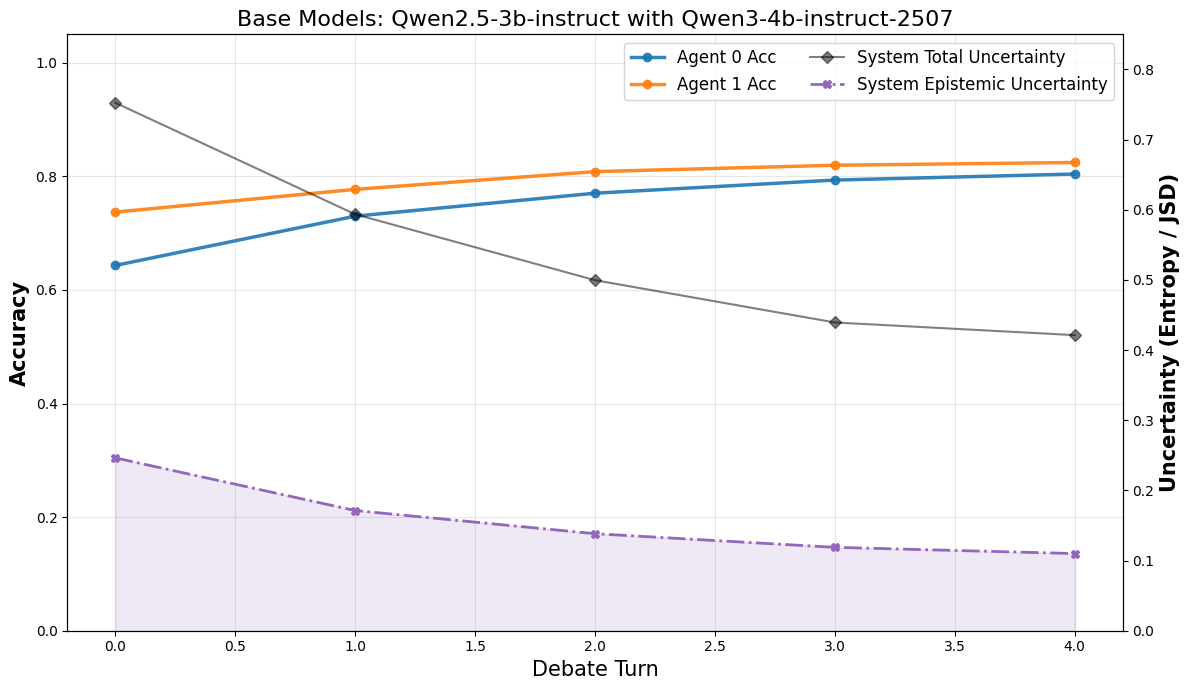
\includegraphics[width=\linewidth]{fig/main_uncertainty/hetero_before.png}
        \caption{基础模型}
    \end{subfigure}

    \vspace{0.3em}

    \begin{subfigure}{0.85\linewidth}
        \centering
        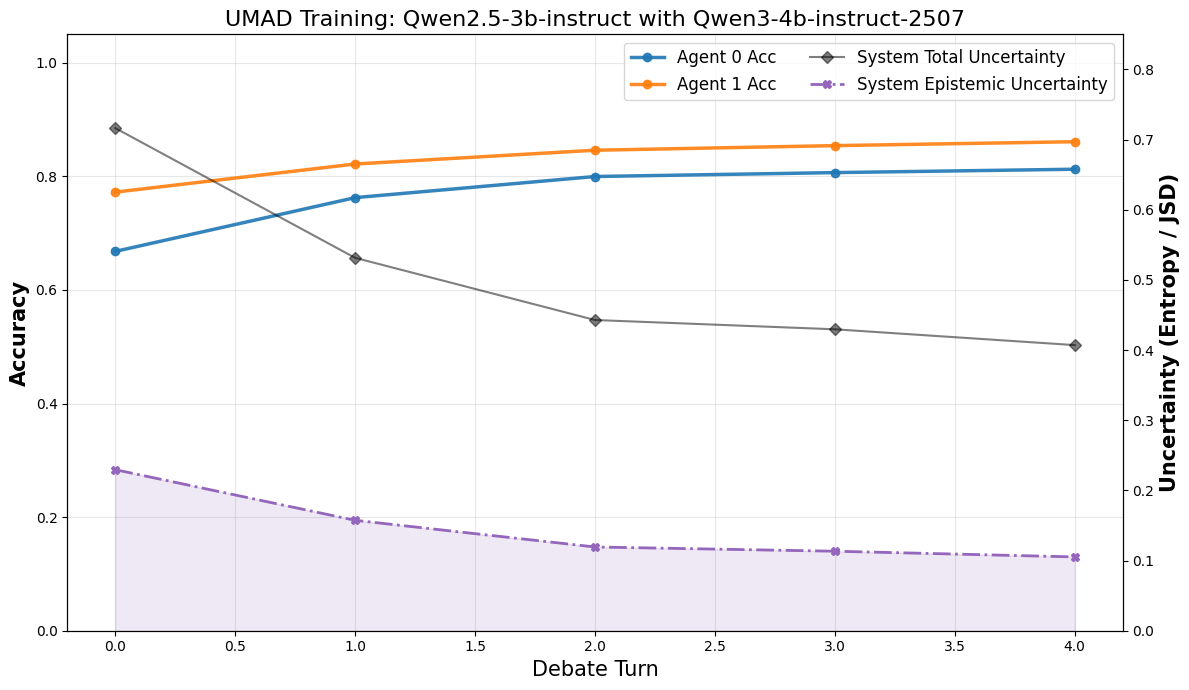
\includegraphics[width=\linewidth]{fig/main_uncertainty/hetero_after.png}
        \caption{UMAD 模型}
    \end{subfigure}

    \vspace{-6pt}
    \caption{不确定性动态（灰色和紫色）与准确率（橙色和蓝色）的对比。UMAD 训练抑制偶然噪声，并提高两个智能体在各轮辩论中的准确率。}
    \label{fig:ablation_uncertainty}
    \vspace{-8pt}
\end{figure}


\section{相关工作}
\textbf{多智能体辩论。}既有 MAD 工作 \cite{du2023improving, liang2024encouraging, chan2024chateval} 表明，相较思维链（CoT）\cite{wei2022chain} 和自洽性 \cite{wang2023selfconsistency} 等单智能体提示方法，迭代辩论能够改善推理。现有研究主要通过工作流设计 \cite{liu2024groupdebate, zhang2025debate4math, maiga2025error, yao2025peacemaker}、通信拓扑优化 \cite{li2024improving, sun2025cortexdebate, eo2025necessary}、模型组合分析 \cite{zhang2025if, smit2023should}，或置信度感知的提示与汇总 \cite{yang2024confidence, chen2024reconcile, lin2025enhancing, yoffe2024debunc} 来改进 MAD。然而，近期研究发现，推理时辩论可能受到谄媚、长上下文漂移以及“共识但不正确”等问题影响 \cite{choi2025debate, pan2025multiagent, yang2025revisiting, wynn2025talk}。不同于依赖冻结模型提示或汇总规则的方法，我们分析辩论期间答案层面的不确定性，并使用不确定性引导的训练信号改善同伴信息利用。

\textbf{MAD 中的多样性与不确定性。}
同期研究也考察了 MAD 中的多样性与不确定性。\citet{zhu2026demystifying} 将 MAD 的失败归因于初始多样性不足和置信度失准，而 \citet{ai2025beyond,li2026dynadebate} 则通过优化汇总或推理路径来提高信息增益。另一些工作指出异构团队存在利用鸿沟和整合折中等局限 \cite{li2026m3mad,pappu2026multi}，或以互补证据解释异构性的作用 \cite{yang2026understanding}。这些工作主要分析推理时行为或汇总协议。相比之下，本文借助偶然控制代理和认知影响代理，将不确定性分解与可训练的辩论行为联系起来，使系统能够主动管理“探索多样同伴观点”与“保持个体推理稳定性”之间的权衡。因此，我们把经验性的辩论启发式转化为形式化、由优化驱动的训练过程。

\textbf{LLM 不确定性与多智能体强化学习。}
不确定性量化已被广泛用于研究 LLM 的可信度 \cite{huang2025look}，包括词元级置信度、语义不确定性 \cite{kuhnsemantic, wang2025measuring}，以及将不确定性拆分为偶然分量和认知分量的贝叶斯分解 \cite{liu2025uncertainty, huang2024survey, geng2024confidencesurvey, abbasi2024believe, jayasekera2025variational, ling2024uncertainty}。相关工作还使用多智能体扰动 \cite{amayuelas2024knowledge} 或微调 \cite{feng2025rethinking} 来引出不确定性信号。另一方面，近期 MARL 方法通过角色设计、策略优化或信用分配来训练基于 LLM 的多智能体系统 \cite{park2025maporl,liao2025marft,liu2025llm,zhao2025stronger}。我们的方法结合这两个方向：利用 MAD 内部的不确定性诊断来设计 MARL 奖励，以稳定单个智能体的推理并促进有用的同伴影响。更多相关工作见附录~\ref{app:more_related}。







\section{结论}
本文从贝叶斯不确定性的视角出发，处理多智能体辩论固有的不稳定与低效问题，尤其是异构设置中的问题。我们发现，性能下降源于偶然噪声失控以及无法有效利用认知分歧。为此，我们提出不确定性引导的 MARL 框架，主动调节内部推理置信度并激励建设性信息交换。该方法带来稳健的性能收益，并防止长轮次辩论中的信念崩溃，从而将 MAD 从脆弱的推理时启发式方法转变为一种稳定、可学习的可靠推理机制。



\clearpage

% Acknowledgements should only appear in the accepted version.
\section*{致谢}
Baoxiang Wang 和 Dan Qiao 的工作得到国家自然科学基金（编号 72394361）及深圳市科技计划（编号 JCYJ20250604141218024、JCYJ20250604141032005）的部分资助。
Wenhao Li 的工作得到国家自然科学基金（编号 62406270）和上海市科委“扬帆计划”（编号 24YF2748800）资助。Fengyu Cai 的工作由德国联邦教育与研究部通过 Software Campus 3.0 项目 ETRAG（资助编号 16IS23067）提供资助。作者衷心感谢香港中文大学（深圳）的 Youliang Yuan、Yajiao Liu、Fei Yu、Xiaoyuan Liu、Jiawei Xu、Yue Lin、Han Wang、Ang Li、Zhongxiang Dai 和 Zhiwei Shang 所提供的深刻讨论与持续支持。
我们也感谢帝国理工学院的 Lihu Chen 在本工作早期开发阶段提供的宝贵反馈。
最后，感谢匿名审稿人提出的建设性意见与建议。

\section*{影响声明}

本工作通过将多智能体辩论建立在贝叶斯框架之上，旨在提高大语言模型的可靠性。我们的方法 UMAD 能够缓解高置信度幻觉，从而支持在数学和科学等关键领域部署可信人工智能。然而，我们也承认，显式优化智能体的“说服力”存在潜在风险：如果将该机制用于主观或敏感领域，理论上可能被滥用于生成看似可信却具有操纵性的内容。未来研究应确保此类能力始终与事实核验严格对齐。此外，我们通过证明高效的短时域训练能够有效泛化到长上下文推理，也回应了多智能体系统的环境成本问题。






\bibliography{example_paper}
\bibliographystyle{icml2026}

%%%%%%%%%%%%%%%%%%%%%%%%%%%%%%%%%%%%%%%%%%%%%%%%%%%%%%%%%%%%%%%%%%%%%%%%%%%%%%%
%%%%%%%%%%%%%%%%%%%%%%%%%%%%%%%%%%%%%%%%%%%%%%%%%%%%%%%%%%%%%%%%%%%%%%%%%%%%%%%
% APPENDIX
%%%%%%%%%%%%%%%%%%%%%%%%%%%%%%%%%%%%%%%%%%%%%%%%%%%%%%%%%%%%%%%%%%%%%%%%%%%%%%%
%%%%%%%%%%%%%%%%%%%%%%%%%%%%%%%%%%%%%%%%%%%%%%%%%%%%%%%%%%%%%%%%%%%%%%%%%%%%%%%
\newpage
\appendix
\onecolumn



\section{更多相关工作}
\label{app:more_related}
\paragraph{多智能体辩论。}
早期 MAD 研究表明，多个 LLM 智能体之间的迭代交互可以引出多样化的解法路径并汇总最终答案，从而改善推理 \cite{du2023improving, liang2024encouraging, chan2024chateval}。后续工作通过任务特定工作流 \cite{liu2024groupdebate, zhang2025debate4math, maiga2025error, yao2025peacemaker}、通信拓扑 \cite{li2024improving, sun2025cortexdebate, eo2025necessary} 和模型组合分析 \cite{zhang2025if, smit2023should} 改进 MAD。另一个研究方向将置信度信号引入辩论：或是在提示中加入同伴置信度 \cite{yang2024confidence, chen2024reconcile}，或是把置信度用作汇总权重 \cite{lin2025enhancing, eo2025necessary, yoffe2024debunc}。然而，近期研究表明，推理时辩论并不总能改善单个智能体的推理。去掉汇总后，同构辩论可能停滞 \cite{choi2025debate}；智能体可能把正确答案改成错误答案 \cite{wynn2025talk}；谄媚或长上下文漂移还可能推动智能体达成表面共识 \cite{pan2025multiagent, yang2025revisiting}。这些发现促使我们关注个体信念的演化，而不是最终汇总准确率。

\paragraph{MAD 中的多样性与不确定性。}
若干同期研究分析了多样性、置信度和不确定性在 MAD 中的作用。\citet{zhu2026demystifying} 认为，初始多样性不足和置信度失准是 MAD 失败的关键原因，并提出文本置信度调制协议来缓解谄媚。为量化干扰集体推理的行为偏差，\citet{choi2025identity} 将辩论动态形式化为身份加权的贝叶斯更新过程，并提出回答匿名化，以强制对智能体身份赋予相等权重。类似地，\citet{ai2025beyond} 研究组合多个回答的高阶汇总规则，而 \citet{li2026dynadebate} 动态生成多样化推理路径，以打破同构推理模式。\citet{li2026m3mad} 等基准研究质疑 MAD 能否在不同领域和模态中持续有效。\citet{pappu2026multi} 进一步表明，由于存在利用鸿沟和整合折中，Graves 智能体团队可能无法充分利用其最强成员。作为补充，\citet{yang2026understanding} 从多样性与互补证据出发，为智能体规模扩展提供了信息论解释。本文的不同之处在于，我们将多样性与不确定性联系到显式的“认知增益与偶然成本”分解，并用该分解设计训练时目标，而不是仅设计推理时协议、匿名化规则或汇总机制。

\paragraph{LLM 中的不确定性量化。}
不确定性量化是评估 LLM 可靠性的核心 \cite{huang2025look}。词元级概率提供了便捷的置信度信号，却往往无法捕捉语义等价性或推理不确定性。语义不确定性方法通过聚类语义等价的生成结果，并在意义而非表面形式上衡量不确定性来解决这一局限 \cite{kuhnsemantic, wang2025measuring}。从汇总角度看，\citet{choi2026modex} 构建相似度图并应用谱聚类，以利用多路径生成之间的语义共识，实现无需评估器的 Best-of-N 选择。贝叶斯不确定性分解进一步区分与模型知识或可约减不确定性相关的认知不确定性，以及与固有歧义或回答变异性相关的偶然不确定性 \cite{liu2025uncertainty, huang2024survey, geng2024confidencesurvey}。这些思想已被用于通用问答 \cite{abbasi2024believe}、上下文学习 \cite{jayasekera2025variational, ling2024uncertainty}、多智能体扰动方法 \cite{amayuelas2024knowledge} 和不确定性感知微调 \cite{feng2025rethinking}。相比之下，我们把不确定性视为 MAD 过程本身的动态属性，其中跨智能体分歧与智能体内部回答不稳定性会随辩论轮次演化。


\paragraph{LLM 中的多智能体强化学习。}
随着基于 LLM 的多智能体系统发展，近期研究已从启发式工作流设计转向可训练的多智能体学习范式。早期探索通常关注交互驱动的数据生成或任务特定角色设计。例如，SPIRAL \cite{liu2025spiral} 表明，推理能力可以从零和博弈的自博弈中涌现，不过它主要关注基于动作的任务，而非数学推理。多智能体微调（MAFT）\cite{subramaniam2025multiagent} 利用多智能体交互收集多样化推理链，用于监督微调。ReMA \cite{wan2025rema} 引入一种在“元思考智能体”与“推理智能体”之间交替的层次架构，将策略监督与具体执行解耦。
更新近的研究把多智能体推理表述为强化学习问题。MAPoRL \cite{park2025maporl} 将辩论形式化为 MARL 过程，并采用 IPPO 风格 \cite{de2020independent} 的训练目标来奖励说服和纠错行为。受 HAPPO \cite{kuba2021trust} 启发，MARFT \cite{liao2025marft} 提出 LaMAS 框架，以改善基于 LLM 的智能体策略更新。其他方法关注信用分配与群体动态。MAGRPO \cite{liu2025llm} 基于 MAPPO \cite{yu2022surprising} 提出集中式团队奖励风格的 MARL 方法；AT-GRPO \cite{zhao2025stronger} 则采用智能体与轮次感知的分组，处理多轮对话中的非平稳性。进一步的研究还探索了 MACA \cite{samanta2025self} 中基于共识的对齐，以及 MPDF \cite{yang2025learning} 中的元策略审议。MARTI \cite{zhang2025marti} 等系统为异步多智能体采样提供了可扩展基础设施。
上述 MARL 研究大多关注同构设置、角色提示或一般信用分配，并未显式分析决定辩论成败的不确定性权衡。同期的 \citet{tang2026value} 提出层次化不确定性度量，并构造由不确定性驱动的策略优化来惩罚行为波动和同伴冲突，以解决辩论崩溃问题。相比之下，UMAD 将 MARL 训练与 MAD 的显式“认知增益与偶然成本”分解联系起来。其认知影响奖励鼓励能够改善同伴推理的回答，而偶然不确定性感知优势塑形则抑制不稳定生成，使训练目标直接对齐于我们分析中识别出的不确定性机制。


\section{理论分析}


\subsection{引理 \ref{lem:log_odds} 的证明}\label{app:proof_lemma1}
\textbf{引理陈述。}
\textit{
假设 $p(h \mid x, c \oplus m) = p(h \mid x, c, m)$ 且 $p(m \mid x, c) > 0$。则：
\[
\log \frac{p(h=1 \mid x, c \oplus m)}{p(h=0 \mid x, c \oplus m)}
=
\log \frac{p(h=1 \mid x, c)}{p(h=0 \mid x, c)}
+
\log \frac{p(m \mid h=1, x, c)}{p(m \mid h=0, x, c)}.
\]
}

\begin{proof}
回顾贝叶斯定理：
\begin{equation}
    p(h \mid x, c, m) = \frac{p(m \mid h, x, c) \cdot p(h \mid x, c)}{p(m \mid x, c)}.
\end{equation}
分别对 $h=1$ 和 $h=0$ 写出该式：
\begin{align}
    p(h=1 \mid x, c, m) &= \frac{p(m \mid h=1, x, c) \cdot p(h=1 \mid x, c)}{p(m \mid x, c)}, \\
    p(h=0 \mid x, c, m) &= \frac{p(m \mid h=0, x, c) \cdot p(h=0 \mid x, c)}{p(m \mid x, c)}.
\end{align}
将第一式除以第二式，边缘似然 $p(m \mid x, c)$ 被约去：
\begin{equation}
    \frac{p(h=1 \mid x, c, m)}{p(h=0 \mid x, c, m)} = \frac{p(h=1 \mid x, c)}{p(h=0 \mid x, c)} \cdot \frac{p(m \mid h=1, x, c)}{p(m \mid h=0, x, c)}.
\end{equation}
两边取自然对数，得到可加的对数优势更新：
\begin{equation}
    \log \frac{p(h=1 \mid x, c \oplus m)}{p(h=0 \mid x, c \oplus m)}
    =
    \log \frac{p(h=1 \mid x, c)}{p(h=0 \mid x, c)}
    +
    \log \frac{p(m \mid h=1, x, c)}{p(m \mid h=0, x, c)}.
\end{equation}
证毕。
\end{proof}

\subsection{命题 \ref{prop:sys_decomp} 的证明}\label{app:proof_prop2}
\textbf{命题陈述。}
\textit{
令 $\mathrm{TU}(t) := H(\bar{p}_t)$。则 $\mathrm{TU}(t) = \mathrm{Sys\mbox{-}EU}(t) + \mathrm{Sys\mbox{-}Cost}(t)$，其中 $\mathrm{Sys\mbox{-}EU}(t) = \mathrm{JSD}(p_{1,t}, \dots, p_{N,t})$，$\mathrm{Sys\mbox{-}Cost}(t) = \frac{1}{N}\sum_i H(p_{i,t})$。
}

\begin{proof}
该结论可由广义 Jensen-Shannon 散度（JSD）的定义直接得到。
对一组分布 $\{p_1, \dots, p_N\}$ 和权重 $\pi_1 = \dots = \pi_N = \frac{1}{N}$，JSD 定义为：
\begin{equation}
    \mathrm{JSD}(p_1, \dots, p_N) := H\left(\sum_{i=1}^N \pi_i p_i\right) - \sum_{i=1}^N \pi_i H(p_i).
\end{equation}
代入记号 $\bar{p}_t = \frac{1}{N}\sum_i p_{i,t}$：
\begin{equation}
    \mathrm{Sys\mbox{-}EU}(t) = H(\bar{p}_t) - \frac{1}{N}\sum_{i=1}^N H(p_{i,t}).
\end{equation}
重新排列各项：
\begin{equation}
    H(\bar{p}_t) = \mathrm{Sys\mbox{-}EU}(t) + \frac{1}{N}\sum_{i=1}^N H(p_{i,t}).
\end{equation}
根据定义，$\mathrm{TU}(t) = H(\bar{p}_t)$ 且 $\mathrm{Sys\mbox{-}Cost}(t) = \frac{1}{N}\sum_i H(p_{i,t})$，故恒等式得证。
\end{proof}



\subsection{定理 \ref{thm:hetero_gain} 的证明}
\label{app:proof_theo3}
\begin{proof}
根据条件互信息的链式法则，两条同构消息提供的认知信息总量可分解为
\begin{align}
I(\varphi; m_{\mathrm{homo}},m'_{\mathrm{homo}} \mid x,c)
&=
I(\varphi; m_{\mathrm{homo}} \mid x,c)
+
I(\varphi; m'_{\mathrm{homo}} \mid x,c,m_{\mathrm{homo}}).
\end{align}
类似地，用一条异构消息替换第二条同构消息，得到
\begin{align}
I(\varphi; m_{\mathrm{homo}},m_{\mathrm{hetero}} \mid x,c)
&=
I(\varphi; m_{\mathrm{homo}} \mid x,c)
+
I(\varphi; m_{\mathrm{hetero}} \mid x,c,m_{\mathrm{homo}}).
\end{align}
两式相减，得到
\begin{align}
& I(\varphi; m_{\mathrm{homo}},m_{\mathrm{hetero}} \mid x,c)
-
I(\varphi; m_{\mathrm{homo}},m'_{\mathrm{homo}} \mid x,c) \nonumber \\
&=
I(\varphi; m_{\mathrm{hetero}} \mid x,c,m_{\mathrm{homo}})
-
I(\varphi; m'_{\mathrm{homo}} \mid x,c,m_{\mathrm{homo}}).
\end{align}
根据假设~\ref{ass:homo_saturation}，
\[
I(\varphi; m'_{\mathrm{homo}} \mid x,c,m_{\mathrm{homo}})
\le
\epsilon_{\mathrm{homo}},
\]
并根据异构互补性条件，
\[
I(\varphi; m_{\mathrm{hetero}} \mid x,c,m_{\mathrm{homo}})
\ge
\epsilon_{\mathrm{homo}}+\Delta.
\]
因此，
\[
I(\varphi; m_{\mathrm{homo}},m_{\mathrm{hetero}} \mid x,c)
-
I(\varphi; m_{\mathrm{homo}},m'_{\mathrm{homo}} \mid x,c)
\ge
\Delta,
\]
命题得证。
\end{proof}



\section{算法与伪代码}



\begin{figure}[t]
    \centering
    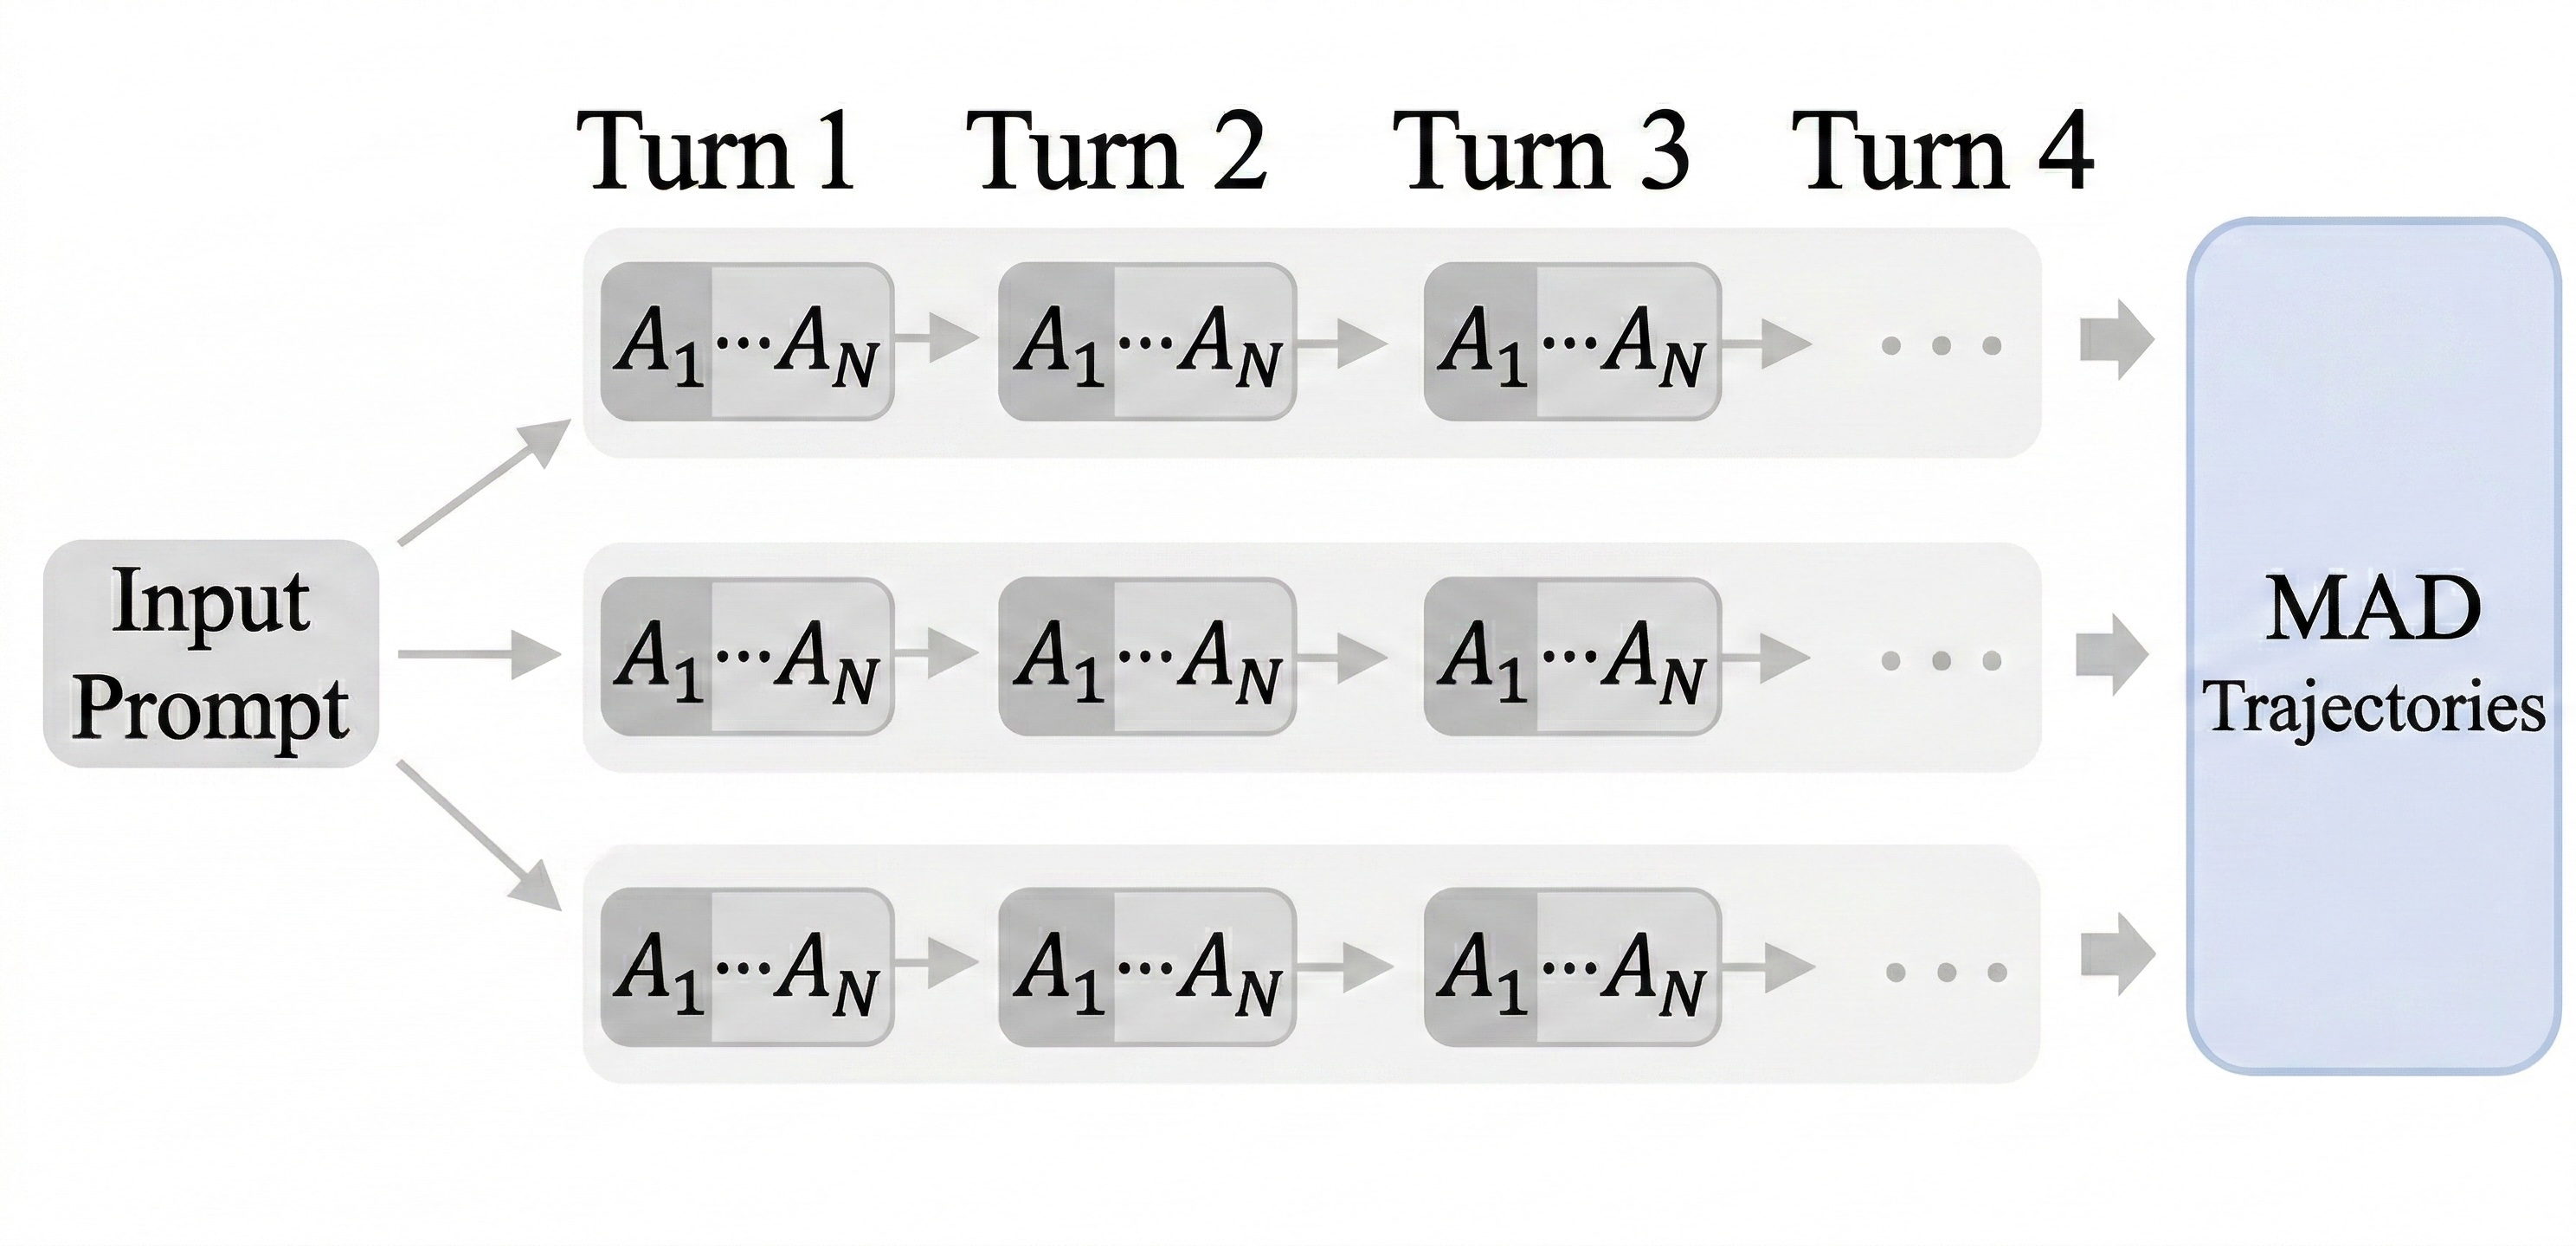
\includegraphics[width=0.5\textwidth]{fig/illustration/debate_rollout.jpg}
    \caption{轨迹级成对辩论采样策略。}
    \label{fig:debate_rollout}
    
\end{figure}


\subsection{多智能体辩论的不确定性量化}

在多智能体辩论中，标准的步骤级分支会导致交互路径组合爆炸，这是 \citet{feng2025gigpo} 指出的一个计算瓶颈。为缓解该问题，我们采用“轨迹级成对辩论采样”策略，如图~\ref{fig:debate_rollout} 所示，维护 $K$ 条并行辩论历史。具体而言，在初始轮（$t=0$），每个参与智能体生成 $K=16$ 条独立轨迹。随后按索引同步这些回答，形成 $K$ 条彼此不同的对话线程，即将智能体 A 的第 $k$ 个回答与智能体 B 的第 $k$ 个回答配对。在后续所有轮次（$t>0$），智能体针对每条已建立的轨迹只生成一次，即 $K=1$。该机制保证 $K$ 条轨迹分别在一致上下文中线性演化，使 GRPO 能够高效运行，而不必承担递归分支带来的指数级开销。


随后，我们汇总最终答案出现的频率，利用这 $K$ 条并行辩论轨迹近似隐式信念分布。为保证稳健性，我们从每条轨迹抽取答案，并合并语义等价的条目。关键在于，不同智能体采样到的答案集合可能互不相交；为使跨智能体散度计算有效，我们将公共支撑集 $\mathcal{Y}_{union}$ 定义为第 $t$ 轮整个团队生成的所有不同答案的并集。然后，在这一全局支撑 $\mathcal{Y}_{union}$ 上计算每个智能体 $i$ 的经验分布 $\hat{p}{i,t}(y)$，并为未观测结果赋予零概率。基于这些对齐后的分布，我们使用团队平均分布 $\bar{p}_t(y) = \frac{1}{N}\sum_{i=1}^N \hat{p}{i,t}(y)$ 量化不确定性。具体而言，\textbf{总不确定性}定义为团队平均分布的熵 $H(\bar{p}_t)$；它进一步分解为\textbf{认知不确定性}与\textbf{偶然不确定性}，分别由智能体间的 Jensen-Shannon 散度和各智能体分布的平均熵衡量。伪代码见表 \ref{alg:mad_uncertainty}。



\begin{algorithm}[p]
   \caption{MAD 不确定性量化}
   \label{alg:mad_uncertainty}
\begin{algorithmic}[1]
   \STATE {\bfseries 输入：}问题数据集 $\mathcal{D}$，智能体 $\{\pi_{\theta_i}\}_{i=1}^N$，最大轮数 $T$，采样数 $K=16$
   \FOR{$\mathcal{D}$ 中的每个问题 $x$}
   \STATE 对所有 $i$ 初始化上下文 $c_{i, 0} \leftarrow \emptyset$
   \FOR{轮次 $t = 1$ 到 $T$}
       \STATE \emph{// 步骤 1：通过采样估计不确定性}
       \FOR{智能体 $i = 1$ 到 $N$}
           \STATE 生成 $K$ 条采样路径：$\{y_{i,t}^{(k)}\}_{k=1}^K \sim \pi_{\theta_i}(\cdot \mid x, c_{i, t-1})$
           \STATE 抽取答案，并按计数频率估计分布 $p_{i,t}(y)$
           \STATE 计算智能体偶然熵：$U_{i,t}^{ale} = H(p_{i,t})$
       \ENDFOR
       
       \STATE \emph{// 步骤 2：计算系统不确定性指标（式 \ref{eq:sys_decomp}）}
       \STATE 计算混合分布：$p_{\mathrm{sys},t}(y) = \frac{1}{N} \sum_{i=1}^N p_{i,t}(y)$
       \STATE \textbf{系统 TU：}$\mathrm{TU}_t = H(p_{\mathrm{sys},t})$
       \STATE \textbf{系统 AU：}$\mathrm{Sys\mbox{-}AU}_t = \frac{1}{N} \sum_{i=1}^N U_{i,t}^{ale}$
       \STATE \textbf{系统 EU（JSD）：}$\mathrm{Sys\mbox{-}EU}_t = \mathrm{TU}_t - \mathrm{Sys\mbox{-}AU}_t$
       
       \STATE \emph{// 步骤 3：进入下一轮（单条轨迹）}
       \FOR{智能体 $i = 1$ 到 $N$}
           \STATE 采样单个回答 $\hat{y}_{i,t} \sim \pi_{\theta_i}(\cdot \mid x, c_{i, t-1})$ \emph{// 或贪心选择}
       \ENDFOR
       \STATE 更新上下文：$c_{i, t} \leftarrow \Phi_i(\{\hat{y}_{j,t}\}_{j=1}^N)$
   \ENDFOR
   \ENDFOR
\end{algorithmic}
\end{algorithm}





\subsection{UMAD 训练算法}

算法 \ref{alg:umad_training} 给出了不确定性引导的多智能体辩论（UMAD）训练框架，它将 GRPO 扩展到协作推理优化。该过程采样一组联合辩论轨迹来估计优势基线，并纳入两项关键调节机制：认知影响内在奖励将后续轮次同伴表现的正向变化归功于相应智能体；偶然不确定性感知优势则根据词元级置信度调节梯度更新。通过整合这些组件，该算法优化策略，在最小化内部推理噪声的同时，最大化为多智能体系统提供的有效信息增益。


\begin{algorithm}[p]
   \caption{不确定性引导的多智能体辩论训练（UMAD）}
   \label{alg:umad_training}
\begin{algorithmic}[1]
   \STATE {\bfseries 输入：}数据集 $\mathcal{D}$，策略 $\pi_{\theta}$，参考模型 $\pi_{ref}$，学习率 $\alpha$，组大小 $G$，辩论轮数 $T_{train}$
   \STATE {\bfseries 超参数：}KL 系数 $\beta$，认知奖励权重 $\eta$
   \WHILE{尚未收敛}
       \STATE 采样一批问题 $x \sim \mathcal{D}$
       \FOR{每个 $x$}
           \STATE \emph{// 通过辩论采样收集轨迹}
           \FOR{组内采样 $g = 1$ 到 $G$}
               \STATE 初始化 $c_{i,0} = \emptyset$
               \FOR{轮次 $t = 1$ 到 $T_{train}$}
                   \FOR{智能体 $i = 1$ 到 $N$}
                       \STATE 采样回答 $y_{i,t} \sim \pi_{\theta}(\cdot \mid x, c_{i,t-1})$
                       \STATE 为 $\hat{\mathcal{U}}_i$ 计算词元级对数概率
                       \STATE 验证正确性 $R_{corr}(y_{i,t}, y^*) \in \{0, 1\}$
                   \ENDFOR
                   \STATE 使用同伴回答更新上下文 $c_t$
               \ENDFOR
           \ENDFOR
           
           \STATE \emph{// 计算奖励与优势}
           \FOR{批次中的每个回答 $(y_{i,t})$}
               \STATE \emph{1. 计算认知内在奖励}
               \STATE 根据下一轮正确性计算同伴平均提升 $\Delta R_{\text{peer}}$
               \STATE 总奖励 $R_{total} = R_{corr} + \eta \cdot \Delta R_{\text{peer}}$（若 $t < T_{train}$）
               
               \STATE \emph{2. 计算组优势}
               \STATE $A_{i,t} = \frac{R_{total} - \text{mean}(R_{group})}{\text{std}(R_{group}) + \epsilon}$
               
               \STATE \emph{3. 应用偶然不确定性加权}
               \STATE $A^{au}_{i,t} = W(\hat{\mathcal{U}}_i) \cdot A_{i,t}$
           \ENDFOR
           
           \STATE \emph{// GRPO 更新}
           \STATE $\mathcal{L} = \mathbb{E} \left[ \min(r A^{au}, \text{clip}(r) A^{au}) - \beta D_{KL}(\pi_\theta \| \pi_{ref}) \right]$
           \STATE 更新 $\theta \leftarrow \theta - \alpha \nabla_\theta \mathcal{L}$
       \ENDFOR
   \ENDWHILE
\end{algorithmic}
\end{algorithm}


\clearpage
\section{实验细节}
\label{app:experiment_details}

\subsection{数据集}

\textbf{MATH} \cite{hendrycks2021measuring}：MATH 数据集包含 12,500 道富有挑战性的竞赛数学题，涵盖代数、几何、组合数学与数论。每道题都提供含多步推理过程的完整逐步解答。

\textbf{GSM8K} \cite{cobbe2021training}：GSM8K 包含 8,500 道小学水平的文字题，重点考察算术与逻辑推理。

\textbf{AMC-23} \cite{amc2023}：该数据集包含从 2023 年美国数学竞赛中选取的 40 道专家级数学题，涵盖代数、组合数学、几何与数论。

\textbf{AIME24（25）} \cite{aops_aime_2024,aops_aime_2025}：每个数据集都包含来自美国数学邀请赛 I 和 II 的 30 道竞赛级问题。



\subsection{LLM 配置与超参数}\label{app:umad_details}

我们基于群组相对策略优化（GRPO）框架 \cite{shao2024deepseekmath} 实现不确定性引导的多智能体辩论（UMAD）训练。训练使用 PyTorch 和 \texttt{verl} \cite{sheng2025hybridflow}，在 $8 \times$ NVIDIA H800 GPU 上进行。生成、优化及 GRPO 算法的详细超参数列于表 \ref{tab:hyperparameters}。

\begin{table}[h]
\centering
\caption{UMAD 训练与推理的详细超参数。}
\label{tab:hyperparameters}
\begin{small}
\begin{tabular}{l|c}
\toprule
\textbf{超参数} & \textbf{取值} \\
\midrule
\multicolumn{2}{c}{\textit{生成配置}} \\
\midrule
训练温度 & $0.8$ \\
推理温度 & $0.6$ \\
Top-p & $0.95$ \\
最大回答长度 & $2,048$ \\
最大提示长度 & $5,120$ \\
\midrule
\multicolumn{2}{c}{\textit{优化器配置}} \\
\midrule
优化器 & Adam \\
学习率 & $1 \times 10^{-6}$ \\
权重衰减 & $0.01$ \\
梯度裁剪范数 & $1.0$ \\
裁剪比率 & 0.2 \\
\midrule
\multicolumn{2}{c}{\textit{GRPO 训练配置}} \\
\midrule
训练 epoch 数 & $2$ \\
训练批大小 & $256$ \\
训练辩论轮数（$T_{train}$） & $2$ \\
评估辩论轮数（$T_{test}$） & $5$ \\
组大小（$G$） & $5$ \\
KL 系数（$\beta$） & $0.001$ \\
认知影响内在奖励（$r_{i,t}^{eu}$） & $0.25$ \\
偶然不确定性优势比率（$\alpha_{au}$） & 0.25 \\
\bottomrule
\end{tabular}
\end{small}
\end{table}

\textbf{奖励配置。}
对于正确性奖励，最终答案正确时赋值 $+1$，否则为 $0$。认知影响内在奖励由 $r_{i,t}^{eu}=0.25$ 控制，以平衡自身正确性与对同伴的说服效果。精确匹配由 MATH 数据集基准 \cite{hendrycks2021measuring} 提供的严格等价性奖励脚本判定。

\textbf{提示格式。}
我们采用数学推理问题的标准聊天模板。前几轮的辩论上下文会追加到用户消息历史中，以确保模型关注同伴的推理路径。详细提示模板见第 \ref{app:prompts} 节。




\subsection{辩论配置}


本文将每个智能体的回答长度设为 2,048，提示长度设为 5,120。通过对不同长度设置的 MAD 进行网格搜索，我们发现 2,048 已足以处理大多数含辩论上下文的问题；8,192 或 32,768 的常规设置只比 2,048 略微准确。考虑计算成本，我们在训练与评估阶段均默认采用 2,048。对于 AIME 问题，我们将回答长度扩展至 4,096、提示长度扩展至 9,216，以避免答案被截断。


\begin{figure}[t]
    \centering
    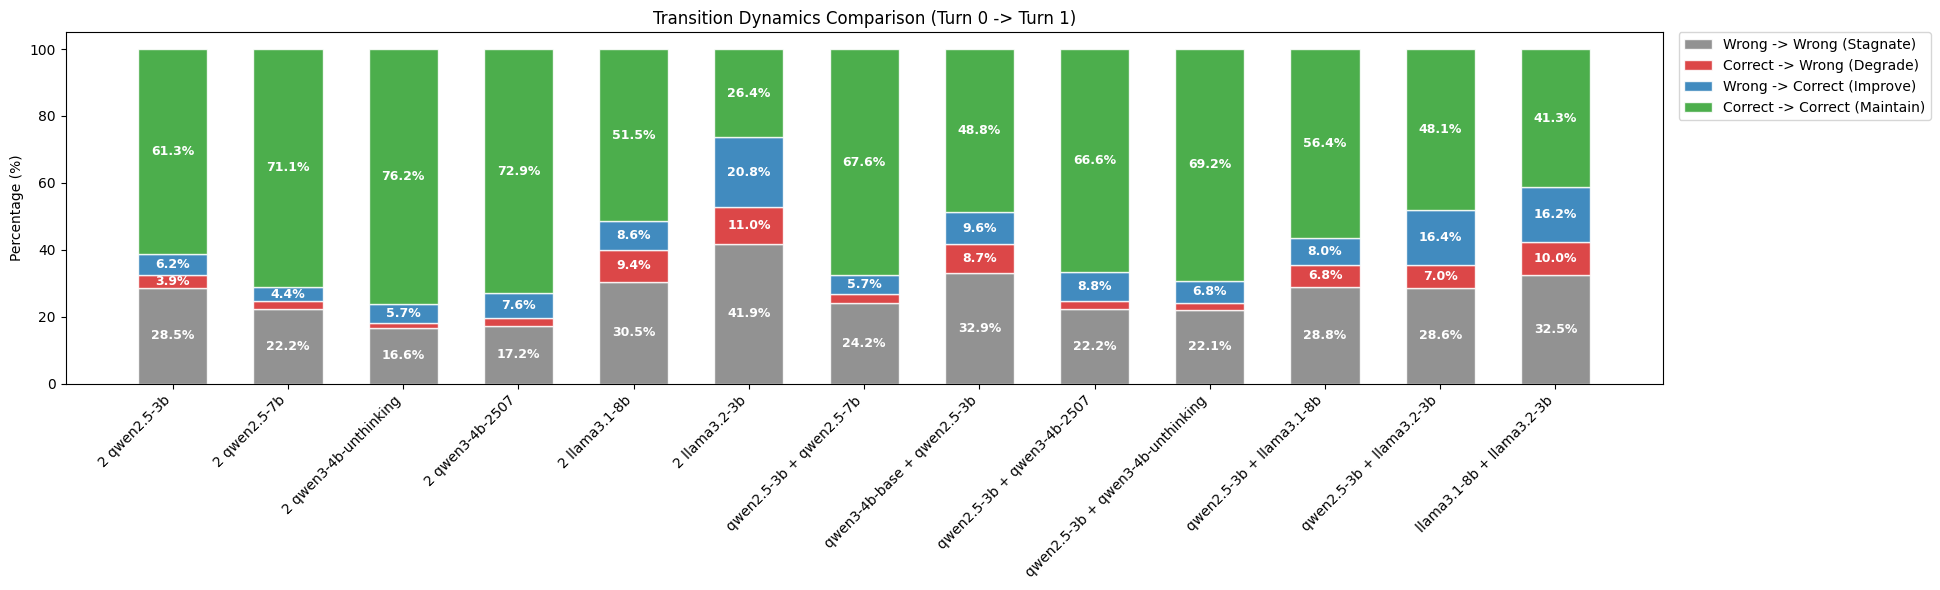
\includegraphics[width=0.95\linewidth]{fig/flip/all_debate_flip.png}
    \caption{同构与异构设置中首轮回答的翻转率。}
    \label{fig:all_flip}
\end{figure}

\subsection{答案翻转动态}\label{subsec:flip_dynamics}



为研究智能体如何应对不断增加的不确定性，我们分析从初始回答到第一轮辩论之间的答案变化（翻转）。结果被划分为四种转变：\textit{正确到正确（C2C）}、\textit{正确到错误（C2W）}、\textit{错误到正确（W2C）}和\textit{错误到错误（W2W）}。\textit{翻转率}定义为两轮之间二值正确性状态发生变化的回答比例，即 $C\to W$ 与 $W\to C$。既有辩论分析广泛使用该统计量来量化稳定性和智能体受同伴影响的程度；我们的定义与这些惯例保持一致，以确保结果可以直接比较。



\begin{figure}[p]
    \centering

    \begin{subfigure}{0.31\linewidth}
        \centering
        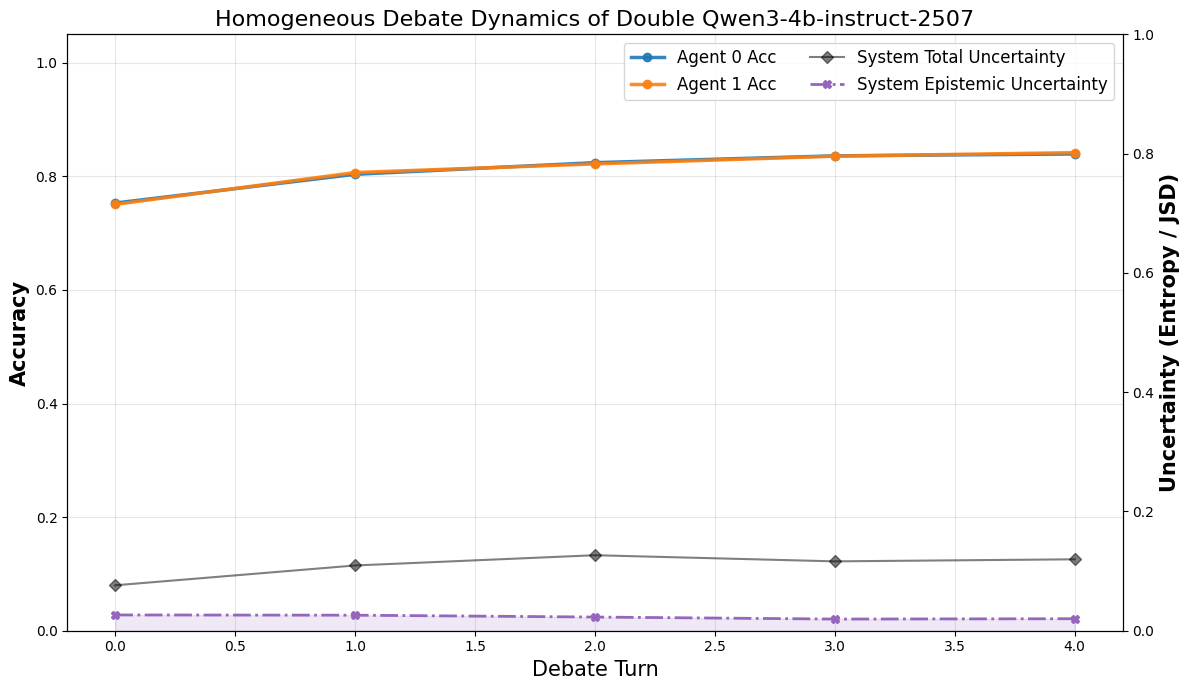
\includegraphics[width=\linewidth]{fig/main_uncertainty/double_2507.png}
        \caption{成功的同构 MAD}
    \end{subfigure}
    \begin{subfigure}{0.31\linewidth}
        \centering
        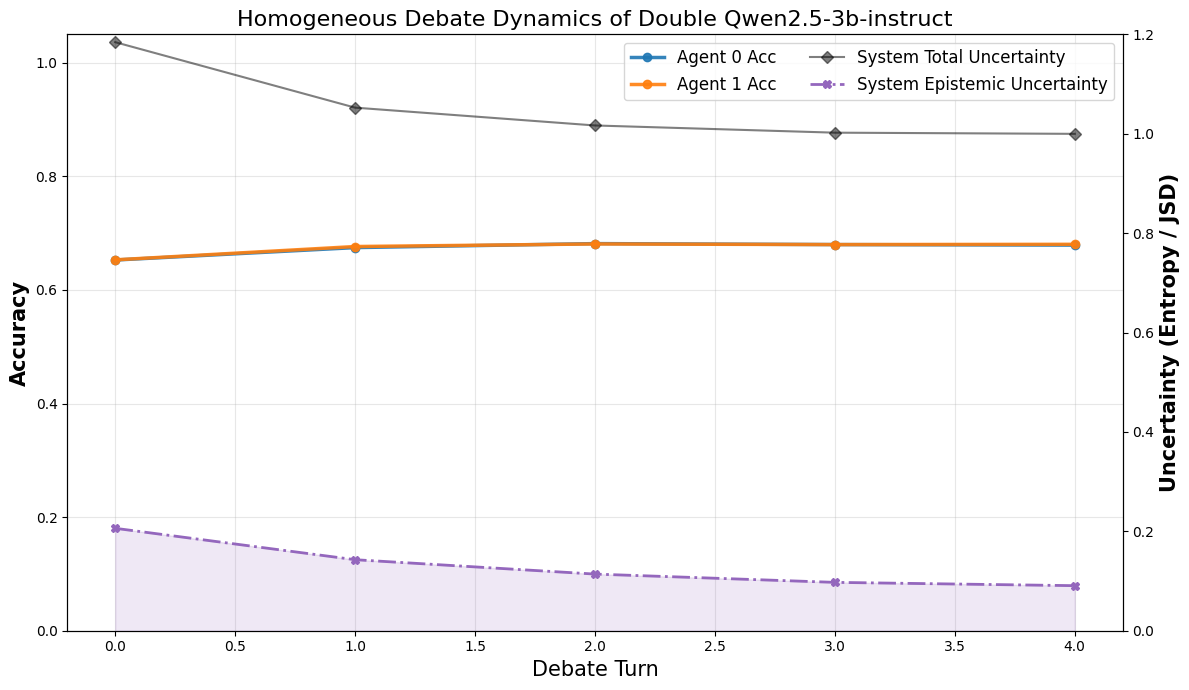
\includegraphics[width=\linewidth]{fig/main_uncertainty/double_2.5-3.png}
        \caption{中性的同构 MAD}
    \end{subfigure}
    \begin{subfigure}{0.31\linewidth}
        \centering
        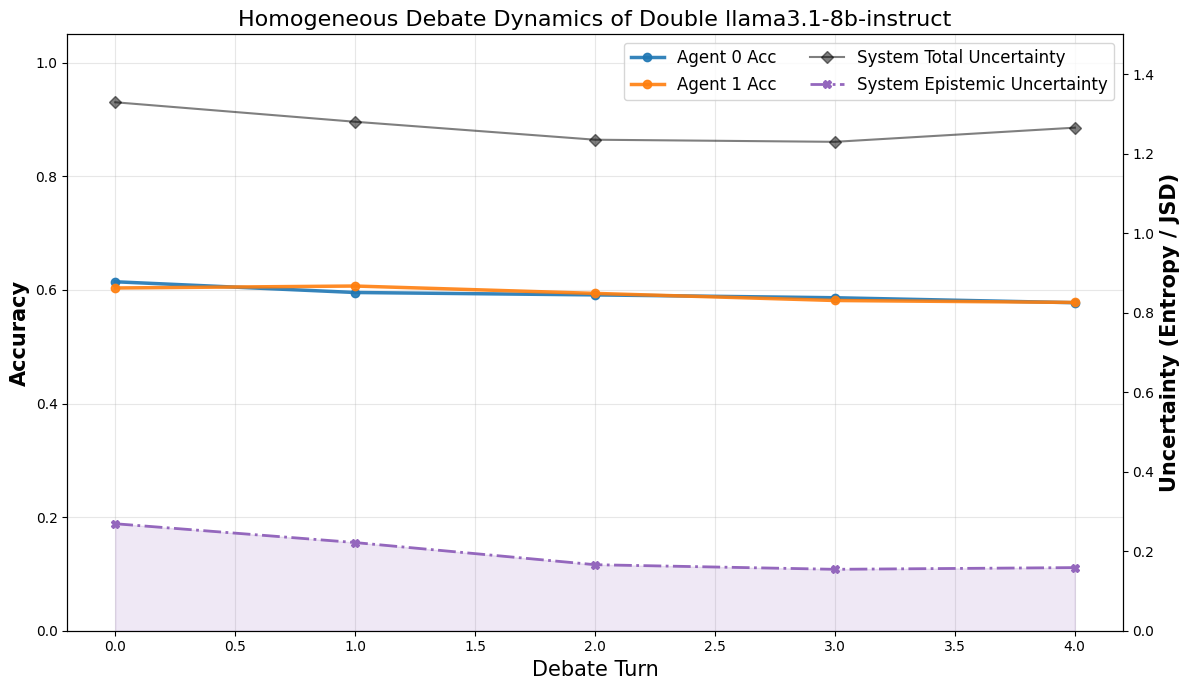
\includegraphics[width=\linewidth]{fig/main_uncertainty/double-llama8.png}
        \caption{失败的同构 MAD}
    \end{subfigure}

    \begin{subfigure}{0.31\linewidth}
        \centering
        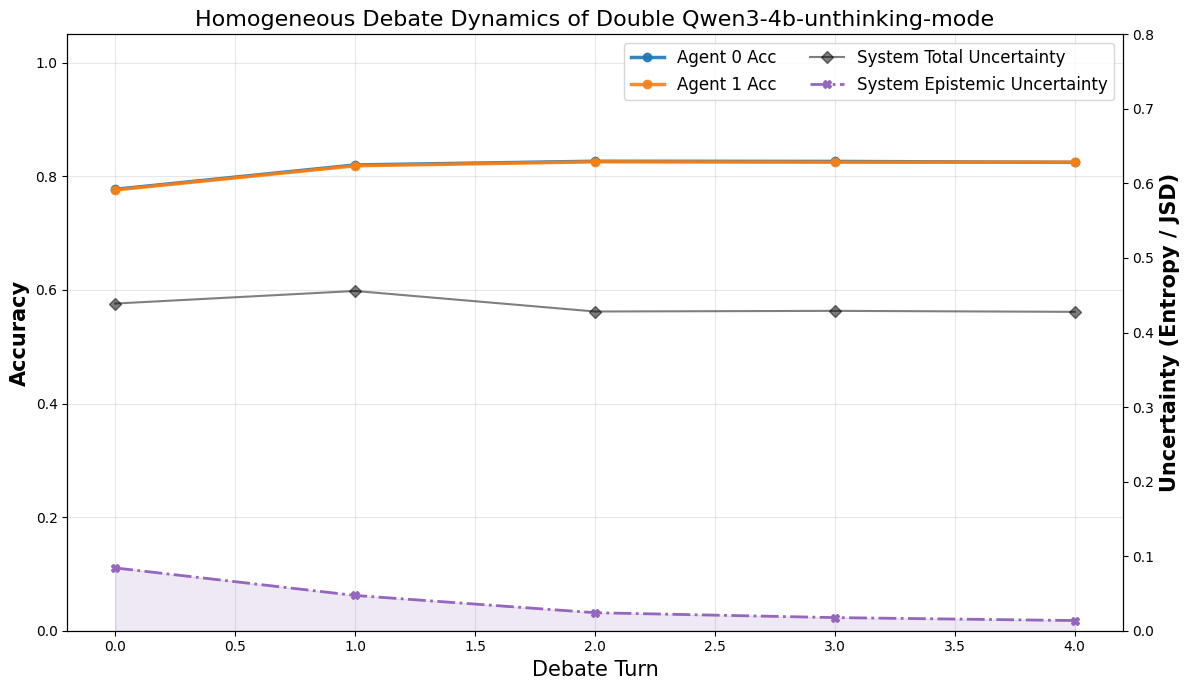
\includegraphics[width=\linewidth]{fig/main_uncertainty/double-4b-unthink.png}
        \caption{成功的同构 MAD}
    \end{subfigure}
    \begin{subfigure}{0.31\linewidth}
        \centering
        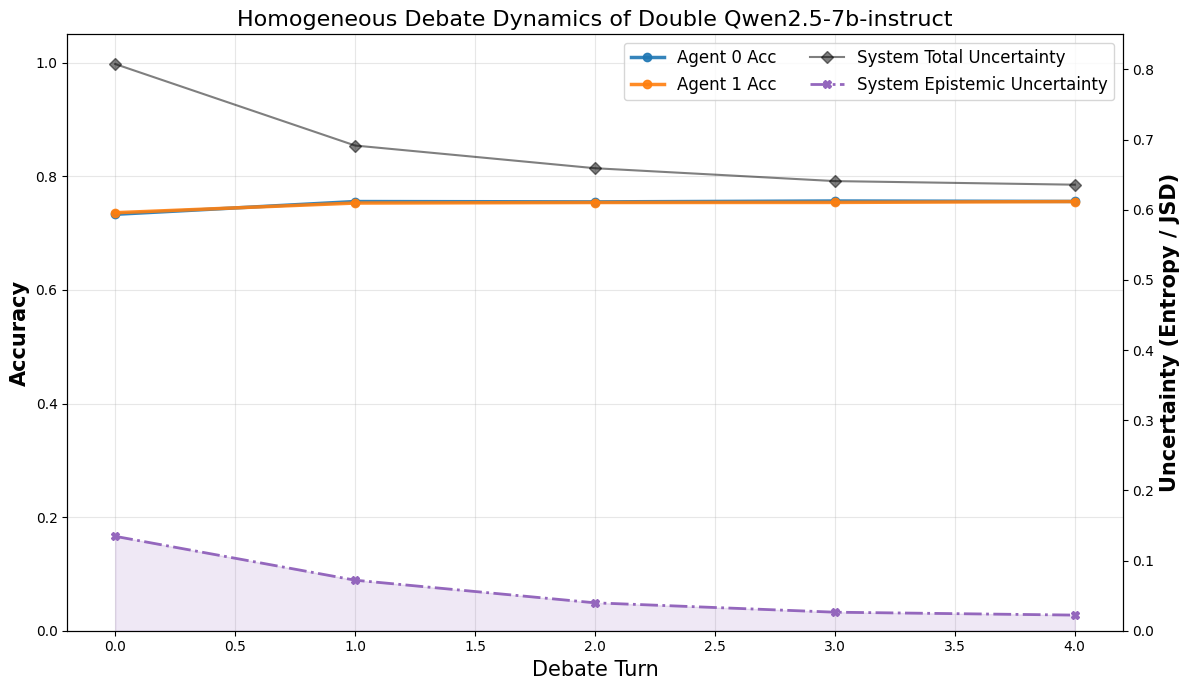
\includegraphics[width=\linewidth]{fig/main_uncertainty/double2.5-7.png}
        \caption{中性的同构 MAD}
    \end{subfigure}
    \begin{subfigure}{0.31\linewidth}
        \centering
        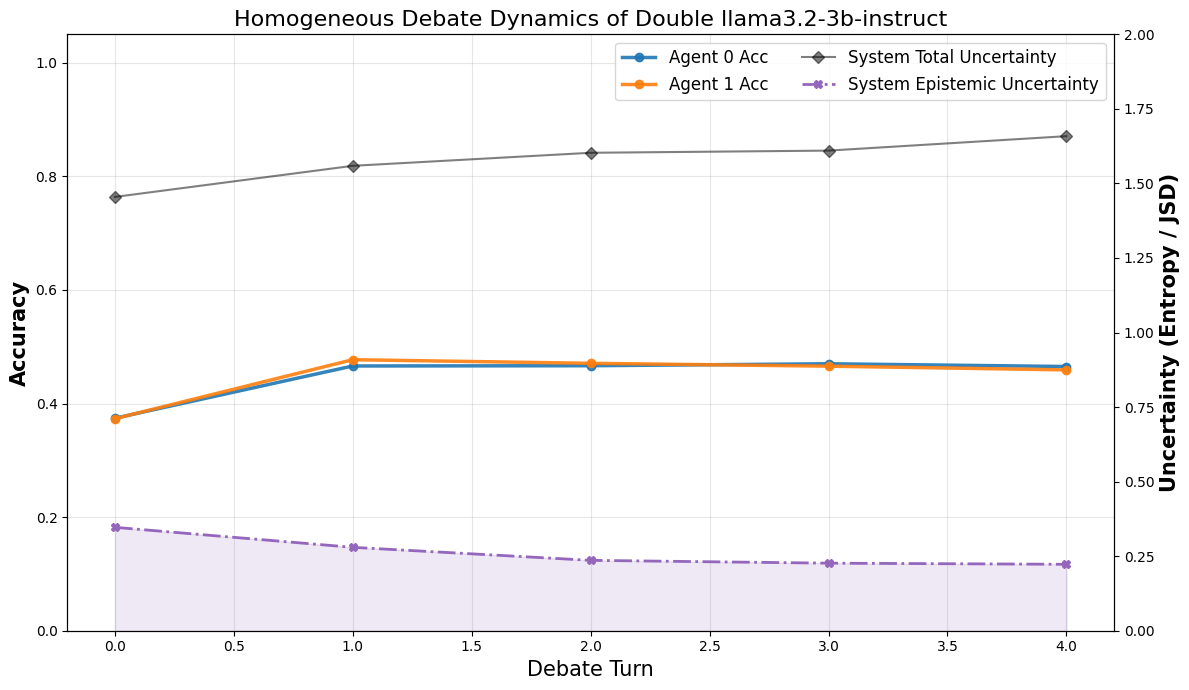
\includegraphics[width=\linewidth]{fig/main_uncertainty/double-llama3.png}
        \caption{成功的同构 MAD}
    \end{subfigure}

    \begin{subfigure}{0.31\linewidth}
        \centering
        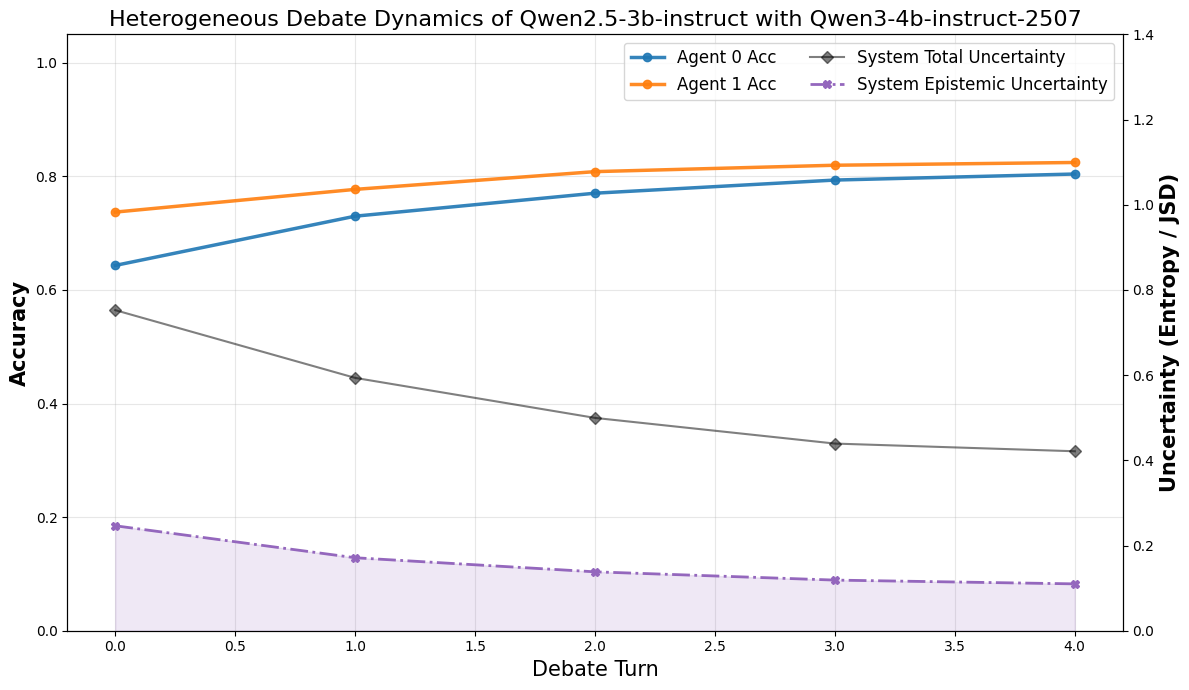
\includegraphics[width=\linewidth]{fig/main_uncertainty/hetero-2.5_2507.png}
        \caption{成功的异构 MAD}
    \end{subfigure}
    \begin{subfigure}{0.31\linewidth}
        \centering
        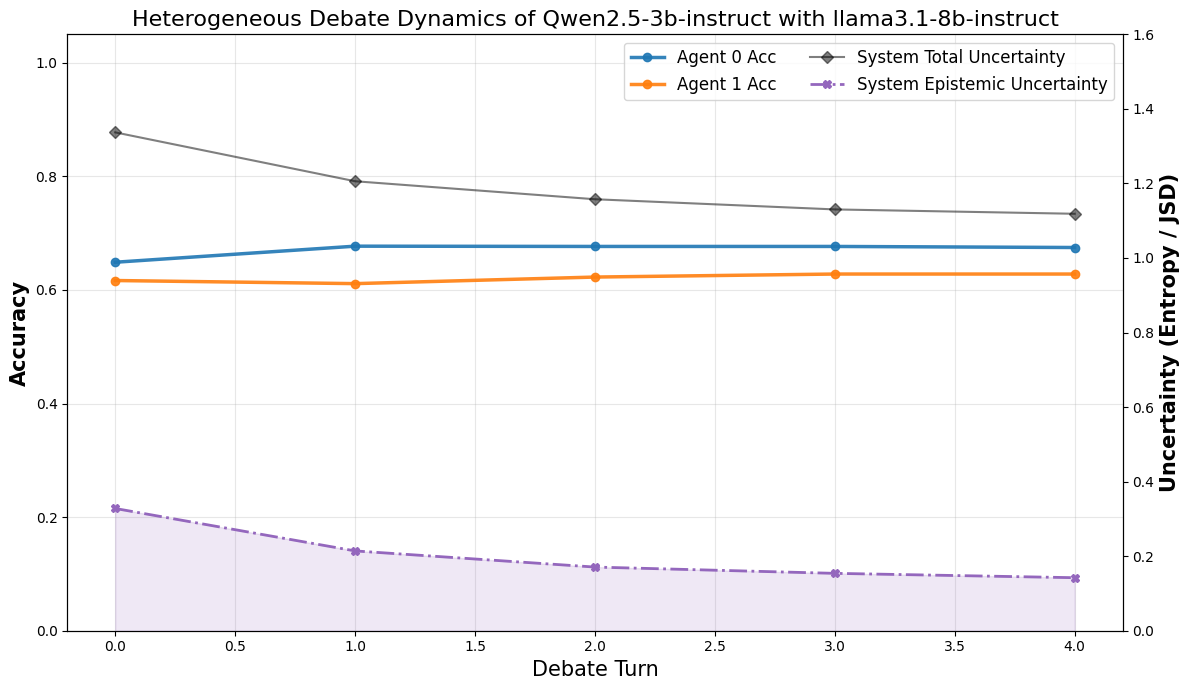
\includegraphics[width=\linewidth]{fig/main_uncertainty/hetero-2.5_llama8.png}
        \caption{中性的异构 MAD}
    \end{subfigure}
    \begin{subfigure}{0.31\linewidth}
        \centering
        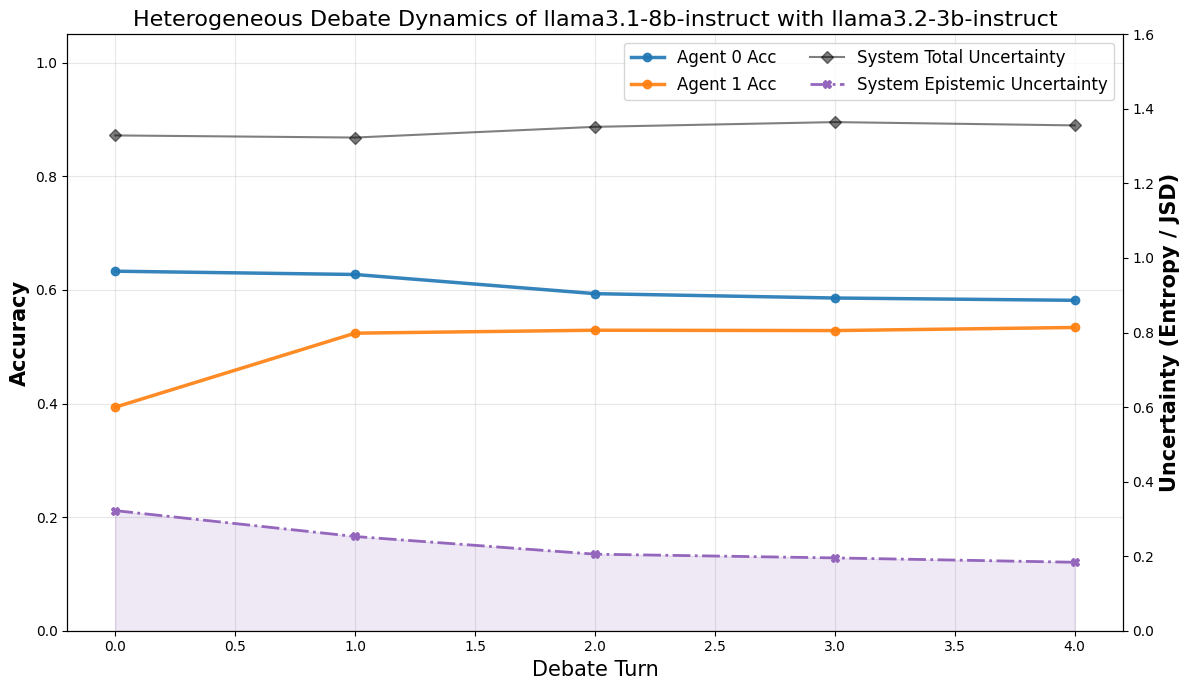
\includegraphics[width=\linewidth]{fig/main_uncertainty/hetero-llama8-llama3.png}
        \caption{失败的异构 MAD}
    \end{subfigure}

    \begin{subfigure}{0.31\linewidth}
        \centering
        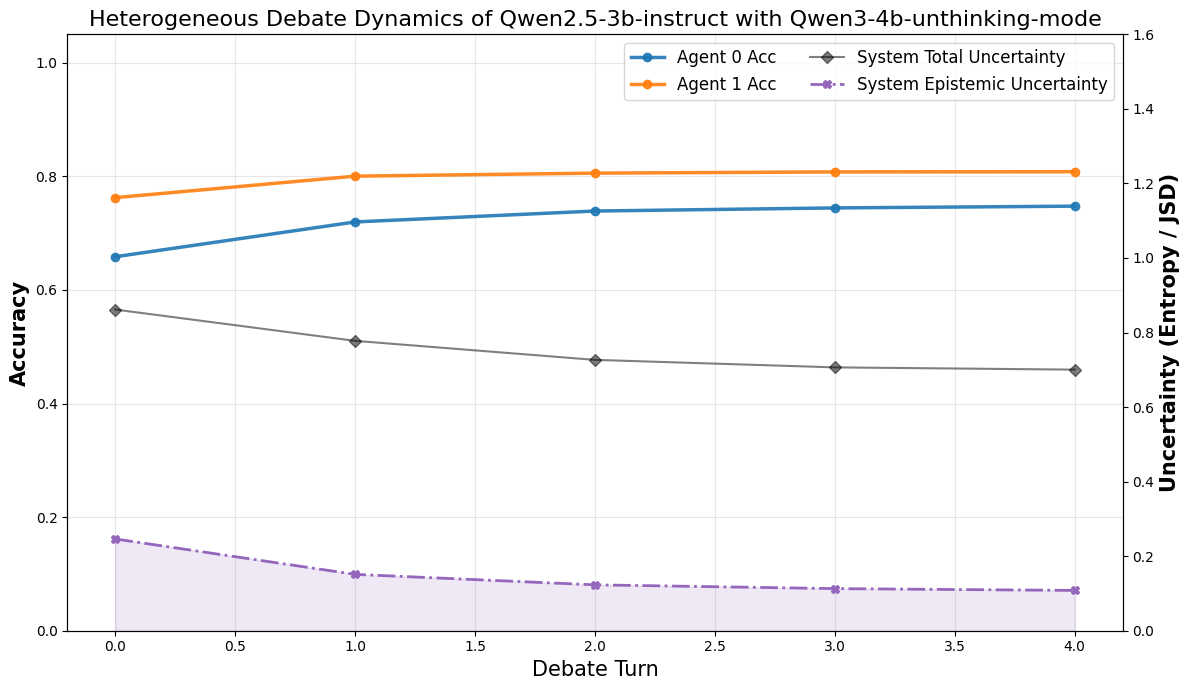
\includegraphics[width=\linewidth]{fig/main_uncertainty/hetero-2.5_unthink.png}
        \caption{成功的异构 MAD}
    \end{subfigure}
    \begin{subfigure}{0.31\linewidth}
        \centering
        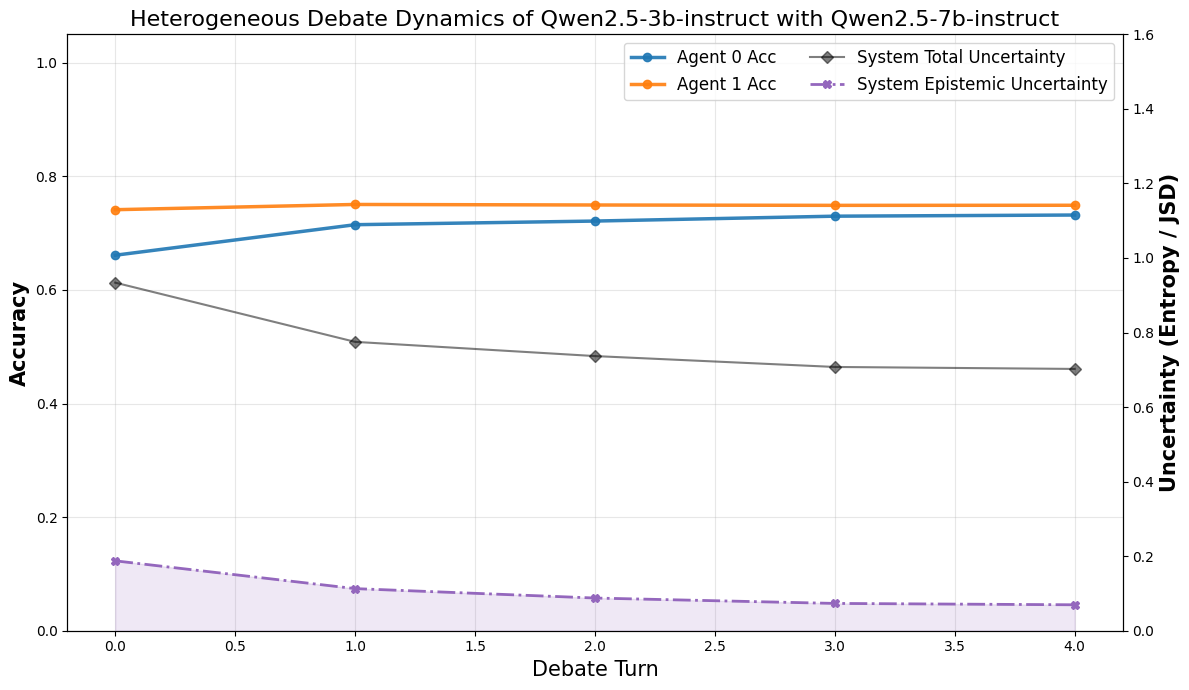
\includegraphics[width=\linewidth]{fig/main_uncertainty/hetero_2.5-7.png}
        \caption{成功的异构 MAD}
    \end{subfigure}
    \begin{subfigure}{0.31\linewidth}
        \centering
        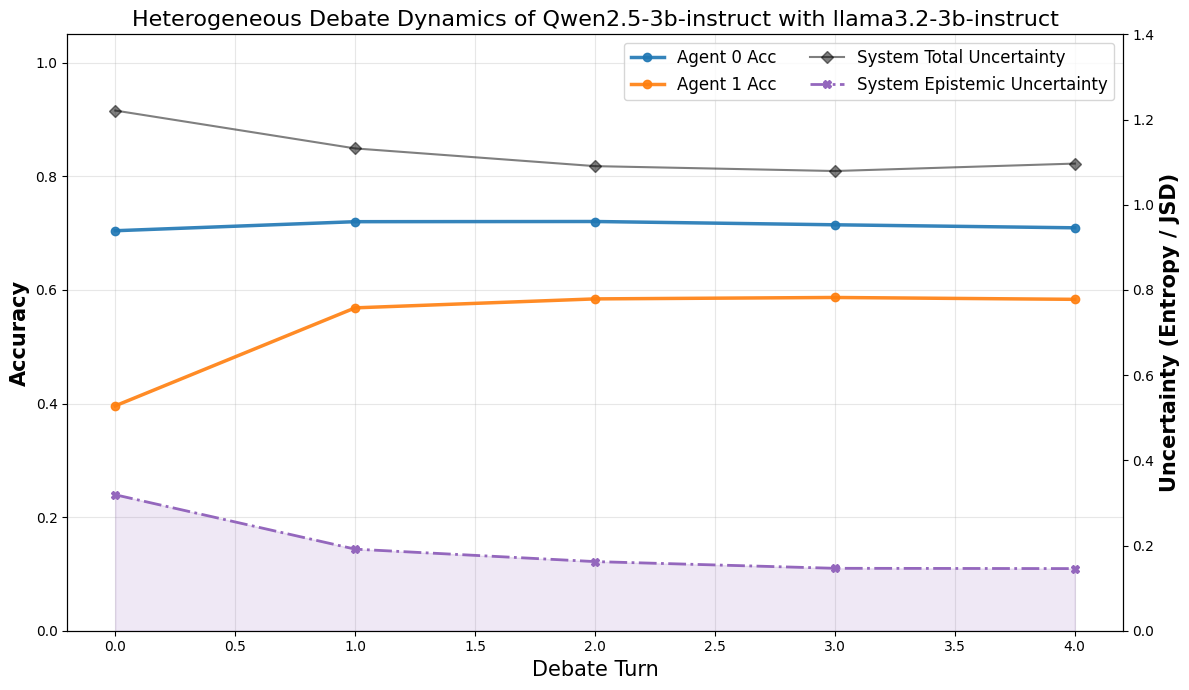
\includegraphics[width=\linewidth]{fig/main_uncertainty/hetero-2.5_llama3.png}
        \caption{成功的异构 MAD}
    \end{subfigure}

    \caption{MAD 中的不确定性分解概览。紫色虚线区域表示系统认知不确定性，灰线表示总不确定性；蓝线和橙线表示测试数据集上的准确率。
    \textbf{上两排：}同构多智能体辩论。
    \textbf{下两排：}异构多智能体辩论。}
    \label{fig:ecac-total}
\end{figure}


图~\ref{fig:all_flip} 展示了同构与异构配对在第一轮的翻转率。首先，强模型的翻转率较低，弱模型的翻转率较高，这与既有辩论研究报告的稳定性差异一致。其次，相对于各自的同构基线，异构配对的翻转率处于中间水平。这些观察与我们的不确定性框架相符：较高翻转率伴随较高预测不确定性，而较低翻转率则反映信念更为集中。







\subsection{系统级不确定性分解结果}\label{app:sys_uncertainty_decomposition}



为验证所提出的框架，我们在 Qwen2.5、Qwen3 和 Llama 模型族的七个模型上开展实验 \cite{yang2024qwen2,yang2025qwen3,grattafiori2024llama}，构成多种同构与异构配置。所有辩论均在 MATH 数据集上进行，智能体数 $N=2$，轮数 $T=5$。关键在于，为弥合理论贝叶斯信念与经验测量之间的差距，我们将采样温度设为 1.0，并让每个智能体在每一轮生成 $K=16$ 条采样路径。由此可以显式计算系统总不确定性，并将其分解为认知不确定性（JSD，表示智能体间冲突）和偶然不确定性（平均熵，表示智能体内部不稳定性）。






\textbf{辩论轨迹分析。}如图~\ref{fig:ecac-total} 所示，我们的实证结果表明，辩论结果由认知消解与偶然控制之间的微妙权衡决定：

\begin{itemize} \item \textbf{普遍共识（认知衰减）：}在所有成功、中性与失败轨迹中，一个普遍趋势是认知不确定性（EU）单调下降。这说明，无论是否符合真实答案，MAD 从根本上都以寻求共识的方式运行，并持续剪除相互冲突的假设。

\item \textbf{通往成功的“偶然壁垒”：}最终准确率的差异主要由偶然不确定性（AU）决定。
\begin{itemize}
    \item \textit{成功模式：}智能体使 AU 保持较低或持续下降，有效锚定正确推理，使其免受噪声干扰。
    \item \textit{失败模式：}这种模式常见于较弱模型（如 Llama 系列），其 AU 不受控制地上升。这说明幻觉强化等“上下文成本”压过了信息交换的收益。
    \item \textit{中性模式：}认知增益恰好被高偶然噪声抵消，形成准确率停滞的平衡状态。
\end{itemize}

\item \textbf{异构优势：}异构配对（如 Qwen-3B 与 Qwen-4B）的初始 EU 显著高于同构配对。更大的“认知差距”提供了更高的改善潜力。当这种高认知潜力在强模型提供的稳定性约束下得以实现时，有效信息增益最大，性能也最优。

\end{itemize}



\begin{table*}[t]
\centering
\caption{异构 MAD 评估在三个随机种子上的均值与标准差。我们报告 $T=1,2,5$ 时单个智能体的 \texttt{pass@1} 准确率，最佳值以粗体标出。}
\label{tab:heterogeneous_three_seed_meanstd}
\resizebox{0.98\textwidth}{!}{
\begin{tabular}{l|l|cc|cc|cc|cc|cc|cc}
\toprule
\multirow{2}{*}{\textbf{方法}} & \multirow{2}{*}{\textbf{轮次}}
& \multicolumn{2}{c|}{\textbf{GSM8K}}
& \multicolumn{2}{c|}{\textbf{MATH500}}
& \multicolumn{2}{c|}{\textbf{AMC23}}
& \multicolumn{2}{c|}{\textbf{AIME24}}
& \multicolumn{2}{c|}{\textbf{AIME25}}
& \multicolumn{2}{c}{\textbf{平均}} \\
& & \textbf{A0} & \textbf{A1}
& \textbf{A0} & \textbf{A1}
& \textbf{A0} & \textbf{A1}
& \textbf{A0} & \textbf{A1}
& \textbf{A0} & \textbf{A1}
& \textbf{A0} & \textbf{A1} \\
\midrule
Full UMAD & $T=1$ & $83.2{\pm}0.9$ & $89.5{\pm}0.7$ & $63.0{\pm}0.7$ & $79.6{\pm}0.9$ & $38.3{\pm}5.2$ & $55.8{\pm}3.8$ & $3.3{\pm}3.3$ & $17.8{\pm}3.8$ & $0.0{\pm}0.0$ & $27.8{\pm}8.4$ & $37.6{\pm}0.6$ & $54.1{\pm}2.1$ \\
Full UMAD & $T=2$ & $90.0{\pm}0.7$ & $90.7{\pm}0.4$ & $83.3{\pm}0.3$ & $82.7{\pm}1.0$ & $65.8{\pm}6.3$ & $62.5{\pm}2.5$ & $20.0{\pm}8.8$ & $28.9{\pm}1.9$ & $26.7{\pm}8.8$ & $35.6{\pm}5.1$ & $57.2{\pm}3.6$ & $60.1{\pm}1.0$ \\
Full UMAD & $T=5$ & $\mathbf{91.1{\pm}0.6}$ & $91.1{\pm}0.2$ & $\mathbf{87.0{\pm}0.7}$ & $86.1{\pm}0.6$ & $\mathbf{80.0{\pm}4.3}$ & $71.7{\pm}3.8$ & $\mathbf{32.2{\pm}6.9}$ & $34.4{\pm}5.1$ & $\mathbf{42.2{\pm}5.1}$ & $\mathbf{45.6{\pm}7.7}$ & $\mathbf{66.5{\pm}2.8}$ & $65.8{\pm}3.1$ \\
\cmidrule(l{0pt}r{0pt}){1-14}
Intrinsic-only & $T=1$ & $83.4{\pm}0.1$ & $89.9{\pm}0.2$ & $65.3{\pm}1.2$ & $76.3{\pm}1.3$ & $39.2{\pm}5.2$ & $59.2{\pm}2.9$ & $1.1{\pm}1.9$ & $18.9{\pm}1.9$ & $3.3{\pm}0.0$ & $21.1{\pm}1.9$ & $38.5{\pm}0.8$ & $53.1{\pm}0.4$ \\
Intrinsic-only & $T=2$ & $86.9{\pm}0.6$ & $91.5{\pm}0.5$ & $75.8{\pm}1.1$ & $83.9{\pm}0.4$ & $57.5{\pm}7.5$ & $72.5{\pm}2.5$ & $14.4{\pm}1.9$ & $32.2{\pm}3.8$ & $10.0{\pm}3.3$ & $35.6{\pm}5.1$ & $48.9{\pm}1.7$ & $63.1{\pm}2.2$ \\
Intrinsic-only & $T=5$ & $88.1{\pm}0.5$ & $91.7{\pm}0.2$ & $78.5{\pm}1.4$ & $85.4{\pm}0.9$ & $63.3{\pm}9.5$ & $83.3{\pm}5.2$ & $22.2{\pm}6.9$ & $35.6{\pm}1.9$ & $15.6{\pm}6.9$ & $37.8{\pm}3.8$ & $53.5{\pm}4.2$ & $66.8{\pm}1.5$ \\
\cmidrule(l{0pt}r{0pt}){1-14}
NLL-only & $T=1$ & $82.8{\pm}1.1$ & $91.0{\pm}0.4$ & $62.1{\pm}0.8$ & $78.3{\pm}0.5$ & $38.3{\pm}8.8$ & $61.7{\pm}5.2$ & $3.3{\pm}3.3$ & $15.6{\pm}3.8$ & $0.0{\pm}0.0$ & $32.2{\pm}1.9$ & $37.3{\pm}1.8$ & $55.7{\pm}1.0$ \\
NLL-only & $T=2$ & $87.1{\pm}0.9$ & $91.0{\pm}0.7$ & $73.2{\pm}0.0$ & $81.9{\pm}1.2$ & $54.2{\pm}3.8$ & $64.2{\pm}6.3$ & $11.1{\pm}7.7$ & $32.2{\pm}5.1$ & $11.1{\pm}1.9$ & $38.9{\pm}10.2$ & $47.3{\pm}2.0$ & $61.6{\pm}1.6$ \\
NLL-only & $T=5$ & $89.4{\pm}1.1$ & $91.4{\pm}0.3$ & $79.6{\pm}0.5$ & $85.4{\pm}0.2$ & $65.8{\pm}1.4$ & $68.3{\pm}2.9$ & $24.4{\pm}11.7$ & $\mathbf{36.7{\pm}6.7}$ & $20.0{\pm}8.8$ & $42.2{\pm}5.1$ & $55.9{\pm}1.2$ & $64.8{\pm}2.2$ \\
\cmidrule(l{0pt}r{0pt}){1-14}
Single-GRPO Pair & $T=1$ & $84.7{\pm}0.4$ & $90.1{\pm}0.3$ & $63.9{\pm}0.1$ & $83.1{\pm}0.1$ & $38.3{\pm}7.2$ & $66.7{\pm}1.4$ & $3.3{\pm}3.3$ & $23.3{\pm}3.3$ & $1.1{\pm}1.9$ & $33.3{\pm}3.3$ & $38.3{\pm}2.3$ & $59.3{\pm}0.8$ \\
Single-GRPO Pair & $T=2$ & $88.1{\pm}0.4$ & $92.1{\pm}0.5$ & $74.2{\pm}2.5$ & $86.9{\pm}0.7$ & $56.7{\pm}2.9$ & $82.5{\pm}4.3$ & $14.4{\pm}6.9$ & $27.8{\pm}5.1$ & $15.6{\pm}1.9$ & $37.8{\pm}1.9$ & $49.8{\pm}1.0$ & $65.4{\pm}0.9$ \\
Single-GRPO Pair & $T=5$ & $90.4{\pm}0.8$ & $\mathbf{92.4{\pm}0.3}$ & $83.4{\pm}1.0$ & $\mathbf{89.5{\pm}1.0}$ & $75.8{\pm}3.8$ & $\mathbf{88.3{\pm}1.4}$ & $22.2{\pm}6.9$ & $30.0{\pm}3.3$ & $28.9{\pm}1.9$ & $38.9{\pm}1.9$ & $60.2{\pm}2.2$ & $\mathbf{67.8{\pm}0.5}$ \\
\bottomrule
\end{tabular}
}
\vspace{-8pt}
\end{table*}


\section{补充消融实验}
\subsection{仅 AU 与仅 EU}\label{app:supply_au_eu}
表~\ref{tab:heterogeneous_three_seed_meanstd} 给出额外消融结果，以分别考察每个不确定性分量在异构 MAD 中的贡献。所有结果都采用与主要实验相同的异构设置，并报告三个评估随机种子上的均值和标准差。这里，\textit{完整 UMAD} 同时使用认知/内在项和基于 NLL 的偶然不确定性代理；\textit{仅内在奖励}去除 AU 代理，只保留认知/内在分量；\textit{仅 NLL} 则只保留基于 NLL 的 AU 代理。我们还加入\textit{单体 GRPO 配对}作为不分解的成对 GRPO 基线。
结果表明，两个不确定性项发挥互补作用。在 $T=5$ 时，完整 UMAD 让较弱智能体 A0 取得最佳平均表现（$66.5{\pm}2.8$），超过仅内在奖励（$53.5{\pm}4.2$）、仅 NLL（$55.9{\pm}1.2$）和单体 GRPO 配对（$60.2{\pm}2.2$）。该优势在 GSM8K、MATH500、AMC23、AIME24 和 AIME25 上一致存在，说明要改善异构辩论中的较弱模型，既需要信息丰富的同伴信号，也需要控制带噪上下文影响。
仅内在奖励和仅 NLL 分别捕捉了部分期望行为，但单独使用均不充分。仅内在奖励在较强智能体 A1 上具有竞争力，$T=5$ 时的平均准确率达到 $66.8{\pm}1.5$，但在 A0 上明显不及完整 UMAD。这说明，在不控制偶然成本的情况下鼓励认知交互，或许能帮助强模型维持准确，却无法可靠地教会弱模型使用同伴信息。相反，仅 NLL 提供了更稳定、面向 AU 的目标，并在 AIME24 上取得 A1 的最佳结果，但它缺少最大化向 A0 传递有用信息所需的显式认知激励。
单体 GRPO 配对在 A1 上表现强劲，$T=5$ 时取得 A1 的最佳平均准确率（$67.8{\pm}0.5$），但在 A0 上仍落后于完整 UMAD。这一模式与主要结果一致：标准成对优化能够保持或改善较强智能体，而不确定性分解则更善于提升非对称辩论中的较弱智能体。总体而言，消融实验支持将 UMAD 设计为一个平衡目标：认知项促进有用分歧与信息交换，AU 代理则抑制不稳定或带噪的辩论动态。











\section{提示示例}\label{app:prompts}

本节给出多智能体辩论过程中使用的提示。这些提示统一用于所有数学推理训练与评估数据集。

\subsection{智能体初始第 0 轮提示}

第一轮中，每个智能体都会收到问题文本和标准的逐步推理指令。最终结果使用格式字符串 \texttt{\textbackslash boxed\{\}} 收尾。

\begin{userchat}
\textbf{系统}（可以根据具体模型的系统指令调整。）\\
你是由阿里云创建的 Qwen。你是一名乐于助人的助手。

\textbf{用户} \\
\texttt{[问题文本]} \\
让我们逐步思考，并将最终答案放在 \texttt{\textbackslash boxed\{\}} 中输出。
\end{userchat}

\subsection{智能体辩论轮提示}

在后续轮次中，每个智能体都会接收上一轮所有智能体的回答，作为额外参考解答。所有智能体的解答都以匿名方式提供，不包含特定智能体身份或有实际含义的角色。由此形成标准化辩论设置，避免角色特定信息或特权信息，并使整个过程始终以原任务和参考解答为基础。指令提示鼓励智能体改进参考解答，但不强制采用固定的反思风格。

\begin{userchat}
\textbf{系统}（可以根据具体模型的系统指令调整。）\\
你是由阿里云创建的 Qwen。你是一名乐于助人的助手。

\textbf{用户} \\
给定以下问题：\texttt{[问题文本]}。\\
现有两个回答：\\
\textbf{智能体 0} 的回答是：\texttt{[智能体 0 的推理与答案]}。\\

\textbf{智能体 1} 的回答是：\texttt{[智能体 1 的推理与答案]}。\\

请仔细审查这些回答并判断哪一个正确。如果其中一个或全部正确，请总结正确回答的推理过程，并给出最终答案。如果二者都错了，请纠正其中的错误，提供一个全新且完整的问题解法，并给出最终答案。让我们逐步思考，并将最终答案放在 \texttt{\textbackslash boxed\{\}} 中输出。
\end{userchat}










\section{更广泛的影响}

本工作提供了一个可操作的贝叶斯不确定性量化框架，推进了对大语言模型（LLM）多智能体交互的理解。我们将重点从表层提示工程转向对内部信念动态的根本调节；由此提出的不确定性引导 MARL（UMAD）方法为构建更可靠、能够自我纠错的推理系统铺平了道路。这对于在科学研究、法律分析等高风险领域部署 LLM 具有更广泛的意义：这些领域中的幻觉风险尤为突出，而“群体智慧”机制对核验至关重要。


\section{计算资源}

所有实验均在高性能计算（HPC）集群上进行。主要硬件配置为单节点，配备 $8 \times$ NVIDIA H800（80GB）GPU。总计算开销如下：

\begin{itemize}

\item \textbf{推理与评估：}多智能体辩论评估包含采样规模 $K=16$ 的偶然不确定性估计，共需要约 40 GPU 小时。

\item \textbf{UMAD 训练：}对于参数规模介于 3B 与 7B 之间的模型，在采样组大小 $G=5$ 的条件下，群组相对策略优化（GRPO）训练阶段消耗 200 至 300 GPU 小时，具体取决于模型规模与上下文长度。

\end{itemize}

\section{生成式人工智能使用声明}

在本文稿的准备过程中，生成式人工智能工具仅用于语言润色，包括改善语法、清晰度和整体行文风格。实验中使用的所有模型均严格遵守各自的开源许可证，所有训练与评估数据均来自公开数据集，从而保证可复现性并遵守合乎伦理的数据使用标准。












\section{局限与未来工作}
UMAD 框架依赖多个智能体之间的多轮交互。尽管我们证明，在短辩论（$T_{\mathrm{train}}=2$）上训练可以泛化到更长的推理时辩论（$T_{\mathrm{test}}=5$），推理成本仍会随智能体数量和辩论轮数近似线性增长，即 $N \cdot T$。未来工作可以探索自适应停止、选择性通信或信念感知路由，以改善准确率与效率之间的权衡。

我们的实证评估聚焦数学推理，因为这类任务的最终答案可验证，答案层面的不确定性也能可靠测量。要将该框架扩展到开放式任务、代码生成或科学推理，需要更稳健的答案等价性检查，以及超越精确匹配验证的不确定性估计方法。

最后，我们的不确定性度量是操作性代理，而非精确的贝叶斯量。我们使用集成答案分布近似系统级预测不确定性，并以词元级负对数似然（NLL）作为回答不稳定性的实用代理。词元级 NLL 虽然计算高效，却并不总与语义不确定性一致，尤其是在模型校准较差，或语义等价解法具有不同表面形式时。未来工作可以引入生成路径的语义聚类、经校准的置信度估计或变分推断，以获得更忠实的不确定性估计。



%%%%%%%%%%%%%%%%%%%%%%%%%%%%%%%%%%%%%%%%%%%%%%%%%%%%%%%%%%%%%%%%%%%%%%%%%%%%%%%
%%%%%%%%%%%%%%%%%%%%%%%%%%%%%%%%%%%%%%%%%%%%%%%%%%%%%%%%%%%%%%%%%%%%%%%%%%%%%%%

\end{document}

% This document was modified from the file originally made available by
% Pat Langley and Andrea Danyluk for ICML-2K. This version was created
% by Iain Murray in 2018, and modified by Alexandre Bouchard in
% 2019 and 2021 and by Csaba Szepesvari, Gang Niu and Sivan Sabato in 2022.
% Modified again in 2023 and 2024 by Sivan Sabato and Jonathan Scarlett.
% Previous contributors include Dan Roy, Lise Getoor and Tobias
% Scheffer, which was slightly modified from the 2010 version by
% Thorsten Joachims & Johannes Fuernkranz, slightly modified from the
% 2009 version by Kiri Wagstaff and Sam Roweis's 2008 version, which is
% slightly modified from Prasad Tadepalli's 2007 version which is a
% lightly changed version of the previous year's version by Andrew
% Moore, which was in turn edited from those of Kristian Kersting and
% Codrina Lauth. Alex Smola contributed to the algorithmic style files.
